\documentclass[11pt, oneside]{article}   	% use "amsart" instead of "article" for AMSLaTeX format
\usepackage{geometry}                		% See geometry.pdf to learn the layout options. There are lots.
\geometry{letterpaper}                   		% ... or a4paper or a5paper or ... 
%\geometry{landscape}                		% Activate for for rotated page geometry
%\usepackage[parfill]{parskip}    		% Activate to begin paragraphs with an empty line rather than an indent
\usepackage{graphicx}				% Use pdf, png, jpg, or eps§ with pdflatex; use eps in DVI mode
\usepackage{amsmath,amssymb}

\usepackage{bm}

\usepackage{hyperref}
\usepackage{cleveref}
\usepackage{setspace}
\usepackage{verbatim}
\usepackage{ifthen}
\usepackage{xcolor}
\usepackage{synttree}
\usepackage{tikz}
\usepackage{subcaption}
\usepackage{algorithm}
\usepackage{algorithmic}
\usepackage{multirow}
\usepackage{hhline}
\usepackage{mathtools}
\usepackage{booktabs}
\usepackage{stackengine}
\usepackage{listings}
\usepackage{graphicx}
\usepackage{amsthm}
\usepackage{sectsty}
\paragraphfont{\normalfont\bfseries\underline}


\definecolor{commentgreen}{RGB}{2,112,10}
\definecolor{eminence}{RGB}{108,48,130}
\definecolor{weborange}{RGB}{255,165,0}
\definecolor{frenchplum}{RGB}{129,20,83}
\lstset{
	language=python,
	frame=tb,
	breaklines=true,
	postbreak=\mbox{\textcolor{red}{$\hookrightarrow$}\space},
	tabsize=4,
	showstringspaces=false,
	numbers=left,
	commentstyle=\color{commentgreen},
	keywordstyle=\color{eminence},
	stringstyle=\color{red},
	basicstyle=\small\ttfamily, % basic font setting
	emph={int,char,double,float,unsigned,void,bool},
	emphstyle={\color{blue}},
	% keyword highlighting
	classoffset=1, % starting new class
	otherkeywords={>,<,.,;,-,!,=,~},
	morekeywords={>,<,.,;,-,!,=,~},
	keywordstyle=\color{weborange},
	classoffset=0,
}
\stackMath
\DeclareMathOperator*{\argmax}{argmax}
\DeclareMathOperator*{\bigtimes}{\times}

% Increase line spacing in algorithms, to increase readability
\usepackage{setspace}
\usepackage{etoolbox}
\AtBeginEnvironment{algorithmic}{\setstretch{1.25}}

\renewcommand{\algorithmicrequire}{\textbf{Input:}}
\renewcommand{\algorithmicensure}{\textbf{Output:}}

\newcommand{\todo}[1]{{\color{red} #1}}
\newcommand{\blue}[1]{{\color{blue} #1}}
\newcommand{\red}[1]{{\color{red} #1}}

\usepackage[normalem]{ulem}

\newcommand{\Bc}{\mathcal{B}}
\newcommand{\Hc}{\mathcal{H}}
\newcommand{\Lc}{\mathcal{L}}
\newcommand{\Mc}{\mathcal{M}}
\newcommand{\Nc}{\mathcal{N}}
\newcommand{\Pc}{\mathcal{P}}
\newcommand{\Rc}{\mathcal{R}}
\newcommand{\Tc}{\mathcal{T}}
\newcommand{\Uc}{\mathcal{U}}
\newcommand{\Yc}{\mathcal{Y}}
\newcommand{\Xc}{\mathcal{X}}
\newcommand{\Rbb}{\mathbb{R}}
\newcommand{\Ebb}{\mathbb{E}}
\newcommand{\Nbb}{\mathbb{N}}
\newcommand{\Pbb}{\mathbb{P}}

\emergencystretch 5em% % To try to force long commands to break line (use \cmdn if not enough)
\newcommand{\cmd}[1]{\texttt{\detokenize{#1}}}			% Write code on the same line
\newcommand{\cmdn}[1]{\newline\texttt{\detokenize{#1}}}	% Write code on a new line

\newcommand{\rank}{\mathrm{rank}}
\DeclareMathOperator{\depth}{depth}
\DeclareMathOperator{\level}{level}

\newtheorem{theorem}{Theorem}[section]
%\newtheorem{remark}[theorem]{Remark}
\newtheorem{example}[theorem]{Example}
\newtheorem{conjecture}[theorem]{Conjecture}
\newtheorem{assumption}[theorem]{Assumption}
%\newtheorem{algorithm}[theorem]{Algorithm}
\newtheorem{definition}[theorem]{Definition}
\newtheorem{lemma}[theorem]{Lemma}\newtheorem{proposition}[theorem]{Proposition}
\newtheorem{question}{Question}
\newtheorem{corollary}{Corollary}

%\usepackage{color}
\usepackage{colortbl}
%\usepackage{multirow}
\definecolor{Gray}{gray}{0.90}

\tikzstyle{active}=[circle,fill=black]

%\setlength{\parindent}{0pt} % No indent

%\onehalfspacing

\newcommand{\showdetails}{show}  % comment this line to hide the details
\theoremstyle{definition}
\makeatletter
\newtheoremstyle{indented}
  {2pt}% space before
  {2pt}% space after
  {\addtolength{\@totalleftmargin}{2.5em}
   \addtolength{\linewidth}{-2.5em}
   \parshape 1 2.5em \linewidth}% body font
  {}% indent
  {\bfseries}% header font
  {.}% punctuation
  {.5em}% after theorem header
  {}% header specification (empty for default)
\makeatother

\theoremstyle{indented}

\newtheorem*{details}{Note}
\newtheorem*{note}{Note}
\newtheorem*{remark}{Remark}
%\newenvironment{details}{}{}
%\newenvironment{details}%
%{%
%	\ifthenelse{\isundefined{\showdetails}}%
%	{\expandafter\comment}%
%	{}%
%	\color{gray}%
%}%
%{%
%	\ifthenelse{\isundefined{\showdetails}}%
%	{\expandafter\endcomment}%
%	{}%
%}

\newcommand{\erwan}[1]{\textcolor{gray}{#1}}
\newcommand{\anthony}[1]{\textcolor{magenta}{#1}}


\title{tensap---A Python Tensor Approximation Package}
\author{Anthony Nouy\footnotemark[1] \and %\;\thanks{Corresponding author, anthony.nouy@ec-nantes.fr} \and 
	    Erwan Grelier\footnotemark[1]} 
\renewcommand{\thefootnote}{\fnsymbol{footnote}}
\footnotetext[1]{Centrale  Nantes, Laboratoire de Math\'ematiques Jean Leray, CNRS UMR 6629}
\renewcommand{\thefootnote}{\fnsymbol{footnote}}
%\date{}							% Activate to display a given date or no date


\begin{document}
\maketitle

\begin{abstract}
This article provides an introduction to tensap (Tensor Approximation Package), which is a Python package for the approximation of functions and tensors, available on GitHub at \url{https://github.com/anthony-nouy/tensap}, or through its GitHub page \url{https://anthony-nouy.github.io/tensap/}.
The package tensap features low-rank tensors (including canonical, tensor train and tree-based tensor formats or tree tensor networks), sparse tensors, polynomials, and allows the plug-in of other approximation tools. It provides different approximation methods based on interpolation, least-squares projection or statistical learning.
\end{abstract}

%\begin{center}
%\huge TEMPORARY VERSION
%\end{center}
\newpage

\tableofcontents



\section*{Introduction}
	tensap (Tensor Approximation Package) is a Python package for the approximation of functions and tensors, available on GitHub at \url{https://github.com/anthony-nouy/tensap}, or through its GitHub page \url{https://anthony-nouy.github.io/tensap/}.
	
	To install from PyPi, run \cmd{pip install tensap}. Alternatively, you can install tensap directly from github by running \\
	\cmd{pip install git+git://github.com/anthony-nouy/tensap@master}.
		
	The package tensap features low-rank tensors (including canonical, tensor-train and tree-based tensor formats or tree tensor networks), sparse tensors, polynomials, and allows the plug-in of other approximation tools. It provides different approximation methods based on interpolation, least-squares projection or statistical learning.
	
	The package is shipped with tutorials showing its main applications. 
	A documentation is also available.
	
	At minimum, tensap requires the packages numpy and scipy. The packages tensorflow and sklearn are required for some applications.
	
	In this document, all Python commands are written using a \cmd{typewriter font}. The quantities in \texttt{typewriter font} are Python objects, whereas the quantities in $math\,font$ are mathematical objects. For better readability, we use the same letter for an object, with different fonts whether we refer to its mathematical definition ($X$) or to its Python implementation (\cmd{X}).
	
%%%% FULLTENSOR	
\section{\cmd{FullTensor}}	
\label{sec:FullTensor}
	A \cmd{FullTensor} \cmd{X} represents an order $d$ tensor $X \in \Rbb^{N_1 \times \cdots \times N_d}$, or multidimensional array of size $N_1\times \hdots \times N_d$. The entries of $X$ are $X_{i_1, \hdots, i_d}$, with $(i_1,\hdots,i_d)$ a tuple of indices, where $i_\nu \in \{0,\hdots,N_\nu-1\}$  is related to the $\nu$-th mode of the tensor. 
\\\par 
	We present in this section how to create a \cmd{FullTensor} using tensap, and several possible operations with such an object. For an introduction to tensor calculus, we refer to the monograph \cite{hackbusch2019tensor}.	
	
For examples of use, see the tutorial file \texttt{tutorials\textbackslash tensor\_algebra\textbackslash tutorial\_FullTensor.py}.
	
	
	\subsection{Creating a \cmd{FullTensor}}
		Provided with an array \cmd{data} of shape \cmd{[N_1, ..., N_d]}, the command \cmd{X = tensap.FullTensor(data)} returns a tensor $X \in \Rbb^{N_1 \times \cdots \times N_d}$, with order \cmd{X.order = d} and shape \cmd{X.shape = (N_1, ..., N_d)}. 
		The number of entries of \cmd{X} is given by $\cmd{X.size = X.storage()} = \prod_{i=1}^d N_i$.
		The number of nonzero entries of \cmd{X} is given by \cmd{X.sparse_storage()}.
		\\\par 
 			It is also possible to generate a \cmd{FullTensor} with entries:
			\begin{itemize}
				\item equal to 0 with \cmd{tensap.FullTensor.zeros([N_1, ..., N_d])},
				\item equal to 1 with \cmd{tensap.FullTensor.ones([N_1, ..., N_d])},
				\item drawn randomly according to the uniform distribution on $[0, 1]$ with \cmd{tensap.FullTensor.rand([N_1, ..., N_d])},
				\item drawn randomly according to the standard gaussian distribution with \cmd{tensap.FullTensor.randn([N_1, ..., N_d])},
				\item different from 0 only on the diagonal, provided in \cmd{diag_data}, with \cmd{tensap.FullTensor.diag(diag_data, d)} (generating a tensor of order d and shape $[N, \hdots, N]$, with $N = $ \cmd{len(diag_data)}),
				\item generated using a provided \cmd{generator} with \cmd{tensap.FullTensor.create(generator, [N_1, ..., N_d])}.
			\end{itemize}
 
	\subsection{Accessing the entries of a \cmd{FullTensor} }\label{sec:subtensor}
		The entries of a tensor \cmd{X} can be accessed with the method \cmd{eval_at_indices}: \cmd{X.eval_at_indices(ind)} returns the entries of $X$ indexed by the list \cmd{ind} containing the indices to access in each dimension.

\paragraph{Extracting diagonal entries.}
For a tensor $X \in \Rbb^{N, \hdots, N}$, the command \cmd{X.eval_diag()} returns the diagonal entries $X_{i, \hdots, i}$, $i = 1, \hdots, N$, of the tensor. The command \cmd{X.eval_diag(dims)} returns the entries $X_{i, \hdots, i}$, with $i$ in \cmd{ind}.

\paragraph{Extracting a sub-tensor.}

			A sub-tensor can be extracted from \cmd{X} with the method \cmd{sub_tensor}: for an order-3 \cmd{FullTensor} \cmd{X} of size $N_1\times N_2 \times N_3$, \cmd{X.sub_tensor([0, 1], ':', 2)} returns a sub-tensor of size $2\times N_2 \times 1$ containing the entries 
			$X_{i_1,i_2,i_3}$ with $i_1\in \{0,1\}$, $0\le i_2 \le N_2-1$ and $i_3=2$.
		
		

		\subsection{Permuting the modes of a \cmd{FullTensor}}
%		\begin{details}
			The methods \cmd{transpose} and \cmd{itranspose} permute the dimensions of a tensor \cmd{X}, given a permutation \cmd{dims} of $\{1, \hdots, d\}$.
			They are such that \cmd{X = X.transpose(dims).itranspose(dims)}.
%		\end{details}



	\subsection{Reshaping  a \cmd{FullTensor}.}
	The command \cmd{X.reshape(shape)} reshapes a \cmd{FullTensor} using a column-major order (e.g. used in Fortran, Matlab, R). It relies on the numpy's reshape function with Fortran-like index (argument \cmd{order='F'}).
	For a tuple $(i_1,\hdots,i_d)$, we define 
	$$\overline{i_1,\hdots,i_d} = i_1 + N_1(i_{2-1}-1) + N_1N_2(i_{3-1}-1) + \hdots + N_1\hdots N_{d-1}(i_d-1) .$$
	A tensor $X$ is be identified with a vector $\mathrm{vec}(X)$ whose entries are  $\mathrm{vec}(X)_{\overline{i_1,\hdots,i_d}}$. This vector can be obtained with the command \cmd{X.reshape(N)} with \cmd{N=numpy.prod(X.shape)}. 


\paragraph{$\alpha$-Matricization.}
		For $\alpha \subset \{1,\hdots,d\}$ an its complementary subset $\alpha^c$ in $\{1,\hdots,d\}$, an  $\alpha$-matricization of a tensor $X$ is a matrix $M$ of size  $(\prod_{i \in \alpha} N_i) \times (\prod_{i \in \alpha^c} N_i)$, such that $X_{i_1,\hdots,i_d} = M_{\overline{i_\alpha},\overline{i_{\alpha^c}}}$ with $i_\alpha = (i_\nu)_{\nu\in \alpha}$. It can be obtained with  \cmd{X.matricize(alpha)}, which returns a \cmd{FullTensor} or order $2$.
		The matricization relies on the method \cmd{reshape}.	



\paragraph{Orthogonalization.} 
		It is possible to obtain a representation of a tensor $X$ such that its $\alpha$-matricization is an orthogonal matrix (i.e. with orthogonal columns) using the method \cmd{X.orth(alpha)}.

	

	\subsection{Norms and singular-values}
	
	\paragraph{Computing the Frobenius norm of a \cmd{FullTensor}.}
		The command \cmd{X.norm()} returns the Frobenius norm $\Vert X \Vert_F$ of $X$, defined by 
		\begin{equation*}
			\Vert X \Vert_F^2 = \sum_{i_1}^{N_1} \cdots \sum_{i_d}^{N_d} X_{i_1, \hdots, i_d}^2.
		\end{equation*}
	
	\paragraph{Computing the $\alpha$-singular values and $\alpha$-principal components  of a \cmd{FullTensor}.}
	For a subset $\alpha \subset \{1, \hdots, d\}$ and its complementary subset $\alpha^c$, the $\alpha$-matricization $M$ of $X$ admits a singular value decomposition
	$$
	M_{i_\alpha,i_{\alpha^c}} = \sum_{k} \sigma^k v^k_{i_\alpha} w^k_{i_\alpha^c}
	$$
	where the $\sigma^k$ are the singular values of $M$ and the $v^k$ the corresponding left singular vectors, or principal components of $M$. 
	They are respectively called the $\alpha$-singular values and $\alpha$-principal components of $X$. 
	The $\alpha$-singular values are obtained with \cmd{X.singular_values()}. The $\alpha$-principal components (and $\alpha$-singular values) are obtained with \cmd{X.alpha_principal_components(alpha)}, which is equivalent to \cmd{X.matricize(alpha).principal_components()}.
		
	\subsection{Operations with \cmd{FullTensor}}\label{sec:operations-fulltensor}
	
	
	\subsubsection{Outer  product. } 
	The outer product $X \circ Y$ of two tensors $X\in \Rbb^{N_1 \times \cdots \times N_d}$ and $Y \in \Rbb^{\hat N_1 \times \cdots \times \hat N_{\hat d}}$ is a tensor $Z \in \Rbb^{N_1 \times \hdots \times N_d \times \hat N_1 \times \cdots \times \hat N_{\hat d}}$ of order $d + \hat d$ with entries 
		$$
		{Z}_{i_1,\hdots,i_d,j_1,\hdots,j_{\hat d}} =  X_{i_1, \hdots,i_ d} Y_{j_1, \hdots, j_{\hat d}}
		$$	
		It is provided by \cmd{X.tensordot(Y, 0)}, similarly to 
 numpy's tensordot function.
	\\
		
	
	
\subsubsection{Kronecker product.} The Kronecker product $X\otimes Y$ of two tensors $X$ and $Y$ of the same order $d=\hat d$  is a tensor $Z$ of size $N_1\hat N_1 \times  \hdots \times N_d \hat N_{\hat d}$ with entries 
	$$
	Z_{\overline{i_1j_1},\hdots,\overline{i_dj_d}} = X_{i_1,\hdots,i_d} Y_{j_1,\hdots,j_d}.
	$$
	 It is given by the command \cmd{kron}, which is similar to numpy's kron function, but for arbitrary tensors.

\subsubsection{Hadamard product.}
The Hadamard (elementwise) product $X \circledast Y$ of two tensors $X$ and $Y$ of the same order and size is obtained through the command  \cmd{__mul__(X,Y)}, which returns a tensor $Z$ with entries 	
$$
Z_{i_1,\hdots,i_d} = X_{i_1,\hdots,i_d} Y_{i_1,\hdots,i_d} 
$$	

\subsubsection{Contracted product.} 
	For $I\subset \{1,\hdots,d\}$ and $J \subset \{1,\hdots,\hat d\}$ with $\#I = \#J$, 
		\cmd{Z = X.tensordot(Y, I, J)} performs the mode $(I,J)$-contracted product of $X$ and $Z$ which is a tensor {Z} of order $d + \hat d - \#I - \#J$ with entries
		\begin{equation*}
			{Z}_{(i_\nu)_{\nu \notin I}, (j_\mu)_{\mu \notin J}} =
	 		\sum_{\substack{i_\nu=1 \\ \nu \in I}}^{N_\nu} \sum_{\substack{j_\mu=1 \\ \mu \in J}}^{N_\mu} 
	 		\prod_{\nu \in I} \prod_{\mu \in J} 
	 		\delta_{i_\nu, j_\mu} X_{i_1, \hdots,i_ d} Y_{j_1, \hdots, j_{\hat d}}
		\end{equation*}
		with $\delta_{i,j}$ the Kronecker delta, that is a contraction  of tensors $X$ and $Y$ along dimensions $I$ of $X$ and $J$ of $Y$.
				 For example, for order-$4$ tensors $X$ and $Y$, \cmd{Z = X.tensordot(Y, [0,1], [1,2])} returns a tensor $Z$ or order $4$ such that 
		$$
		Z_{i_3,i_4,j_1,j_4} = \sum_{i_1,i_2} X_{i_1,i_2,i_3,i_4} Y_{j_1,i_1,i_2,j_4} .
		$$
		The method \cmd{tensordot_eval_diag} provides the diagonal (or entries with equal pairs of indices) of the result of the method \cmd{tensor_dot}, but at a cost lower than when using \cmd{X.tensordot(Y, I, J).eval_diag()}. 
		\\
	For example, for order-$4$ tensors $X$ and $Y$,  \\
	\cmd{X.tensordot_eval_diag(Y,[0,1],[1,2],[2,3],[0,3])} returns the diagonal of $Z$, i.e. an order-one tensor $M$ with entries
$$M_k = Z_{k,k,k,k} = \sum_{i_1,i_2} X_{i_1,i_2,k,k} Y_{k,i_1,i_2,k}  $$
 \cmd{X.tensordot_eval_diag(Y,[0,1],[1,2],[2,3],[0,3],diag = True)} returns a tensor $M$ of order $2$ with entries
$$M_{k_1,k_2} = Z_{k_1,k_2,k_1,k_2} = \sum_{i_1,i_2} X_{i_1,i_2,k_1,k_3} Y_{k,i_1,i_2,k}  $$
\cmd{X.tensordot_eval_diag(Y,[0,1],[1,2],[2],[0])} returns the diagonal of $Z$, i.e. a tensor $M$ of order $3$ $v$ with entries
$$M_{k,i_4,j_4} = Z_{k,i_4,k,j_4} = \sum_{i_1,i_2} X_{i_1,i_2,k,i_4} Y_{k,i_1,i_2,j_4}  $$



\subsubsection{Dot product.}	
The dot product of two tensors $X$ and $Y$ with same shape $[N_1, \hdots, N_d]$, defined by
		\begin{equation}
			( X, Y ) = \sum_{\substack{i_\nu = 1 \\ \nu = 1, \hdots, d}}^{N_\nu} X_{i_1, \hdots, i_d} Y_{i_1, \hdots, i_d},
		\end{equation} 
		can be obtained with \cmd{X.dot(Y)}. It is equivalent to \cmd{X.tensordot(Y, range(X.order), range(Y.order))}.
			
			
	\subsubsection{Contractions with  matrices or vectors}
		
			Given a tensor $X$ and a list of matrices $M = [M^1, ..., M^d]$, the command \cmd{Z = X.tensor_matrix_product(M)} returns an order-d tensor $Z$ whose entries are
			\begin{equation*}
				Z_{i_1, \hdots, i_d} = \sum_{\substack{k_\nu = 1 \\ \nu = 1, \hdots, d}}^{N_\nu} X_{k_1, \hdots, k_d} \prod_{\nu = 1}^d M^\nu_{i_\nu, k_\nu}
			\end{equation*}
			The same method exists for vectors instead of matrices: \cmd{tensor_vector_product}.
			Similarly to \cmd{tensordot_eval_diag}, the method \cmd{tensor_matrix_product_eval_diag} evaluates the diagonal of the result of \cmd{tensor_matrix_product}, with a lower cost.
	

	
%\todo{\cmd{__pow__}}


\section{Tensor formats}

Here we present tensor formats available in tensap, which are structured formats of tensors in $\mathbb{R}^{N_1\times \hdots \times N_d}.$ For a detailed description of methods, see the description of the corresponding methods for \cmd{FullTensor} in \Cref{sec:FullTensor}. For an introduction to tensor formats, we refer to the monograph \cite{hackbusch2019tensor} and the survey \cite{nouy:2017_morbook}.		

% CANONICAL TENSOR
	\subsection{\cmd{CanonicalTensor}}
		The entries of an order-$d$ tensor $X \in \Rbb^{N_1 \times \cdots \times N_d}$ in canonical format can be written
		\begin{equation*}
		\label{eq:CanonicalTensor}
			X_{i_1, \hdots, i_d} = \sum_{k=1}^r C_k U^1_{i_1, k} \cdots U^d_{i_d, k},
		\end{equation*}
		with $r$ the canonical rank, and where the $U_\nu = (U^\nu_{i_\nu, k})_{1\le i_\nu \le N_\nu , 1\le k \le r}$ are order-two tensors.
		
		\paragraph{Creating a \cmd{CanonicalTensor}.}
			To create a canonical tensor in tensap, one can use the command \cmd{tensap.CanonicalTensor(C, U)}, where \cmd{C} contains the  $(C_k)_{k=1}^d$, and \cmd{U} is a list containing the  $U^\nu$, $1\le \nu\le d$.
			
			The storage complexity of such a tensor, obtained with \cmd{X.storage()}, is equal to $r(1 + N_1 + \cdots + N_d)$.
\\			
				It is also possible to generate a \cmd{CanonicalTensor} with entries
				\begin{itemize}
					\item equal to 0 with \cmd{tensap.CanonicalTensor.zeros(r, [N_1, ..., N_d])},
					\item equal to 1 with \cmd{tensap.CanonicalTensor.ones(r, [N_1, ..., N_d])},
					\item drawn randomly according to the uniform distribution on $[0, 1]$ with \cmd{tensap.CanonicalTensor.rand(r, [N_1, ..., N_d])},
					\item drawn randomly according to the standard gaussian distribution with \cmd{tensap.CanonicalTensor.randn(r, [N_1, ..., N_d])},
					\item generated using a provided \cmd{generator} with \cmd{tensap.CanonicalTensor.create} \cmd{(generator, r, [N_1, ..., N_d])}.
				\end{itemize}
		
		\paragraph{Converting a \cmd{CanonicalTensor} to a \cmd{FullTensor}.}
			A \cmd{CanonicalTensor} \cmd{X} can be converted to a \cmd{FullTensor} (introduced in Section \ref{sec:FullTensor}) with the command \cmd{X.full()}.
		
		\paragraph{Converting a \cmd{CanonicalTensor} to a \cmd{TreeBasedTensor}.}
			A \cmd{CanonicalTensor} \cmd{X} can be converted to a \cmd{TreeBasedTensor} (introduced in Section \ref{sec:TreeBasedTensor}) with the command \cmd{X.tree_based_tensor(tree, is_active_node)}, with \cmd{tree} a \cmd{DimensionTree} object, and \cmd{is_active_node} a list or array of booleans indicating if each node of the tree is active.
		
		\paragraph{Accessing the diagonal of a \cmd{CanonicalTensor}.}			
			For a canonical tensor $X \in \Rbb^{N \times \hdots \times N}$, the command \cmd{X.eval_diag()} returns the diagonal $X_{i, \hdots, i}$, $i = 1, \hdots, N$, of the tensor. 
			The method \cmd{eval_diag} can also be used to evaluate the diagonal in a subset of dimensions \cmd{dims} of the tensor with \cmd{X.eval_diag(dims)}, which returns a \cmd{CanonicalTensor}.
		
		\paragraph{Computing the Frobenius norm of a \cmd{CanonicalTensor}.}
			The command \cmd{X.norm()} returns the Frobenius norm of $X$.			The Frobenius norm of $X$ is equal to the Frobenius norm of its core $C$ if \cmd{X.is_orth} is \cmd{True}.
			
		\paragraph{Computing the derivative of \cmd{CanonicalTensor} with respect to one of its parameters.}
			Given an order-$d$ canonical tensor $X$ in $\Rbb^{N \times \cdots \times N}$, the command \cmd{X.parameter_gradient_eval_diag(k)}, for $1 \leq k \leq d$, returns the derivative
			\begin{equation*}
				\left.\frac{\partial X_{i_1, \hdots, i_d}}{\partial U^k}\right|_{i_1=\cdots=i_d=i}, \; i = 1, \hdots, N.
			\end{equation*}
			
			The derivative of $X$ with respect to its core $C$, that writes
			\begin{equation*}
				\left.\frac{\partial X_{i_1, \hdots, i_d}}{\partial C}\right|_{i_1=\cdots=i_d=i}, \; i = 1, \hdots, N,
			\end{equation*}
			is obtained with \cmd{X.parameter_gradient_eval_diag(d+1)}.
			
			The method \cmd{parameter_gradient_eval_diag} is used in the statistical learning algorithms presented in Section \ref{sec:TensorLearning}.
		
		\paragraph{Performing operations with \cmd{CanonicalTensor}.}
		Some operations between tensors are implemented for \cmd{DiagonalTensor} (see \Cref{sec:operations-fulltensor} for a detailed description of the operations): 
the Kronecker product with \cmd{kron}, the contraction with matrices  with \cmd{tensor_matrix_product}, the evaluation of the diagonal of a contraction with matrices with \cmd{tensor_matrix_product_eval_diag}, the dot product with \cmd{dot}. 
	
		
			Given a tensor $X$ and a list of matrices $M = [M^1, ..., M^d]$, the command \cmd{Z = X.tensor_matrix_product(M)} returns an order-d tensor $Z$ whose entries are
			\begin{equation*}
			Z_{i_1, \hdots, i_d} = \sum_{k=1}^r \sum_{\substack{k_\nu = 1 \\ \nu = 1, \hdots, d}}^{N_\nu} C_k U^1_{k_1, k} \cdots U^d_{k_d, k} \prod_{\nu = 1}^d M^\nu_{i_\nu, k_\nu}
			\end{equation*}
			The method \cmd{tensor_matrix_product_eval_diag} evaluates the diagonal of the result of \cmd{tensor_matrix_product}.
			
			The dot product of two canonical tensors $X$ and $Y$ with same shape $[N_1, \hdots, N_d]$ can be obtained with \cmd{X.dot(Y)}.
		
		
%% DIAGONAL TENSOR


	\subsection{\cmd{DiagonalTensor}}
		A diagonal tensor $X \in \Rbb^{N_1 \times \cdots \times N_d}$ is a tensor whose entries $X_{i_1, \hdots, i_d}$ are non-zero only if $i_1 = \cdots = i_d$.
		
		\paragraph{Creating a \cmd{DiagonalTensor}.}
			To create a diagonal tensor in tensap, one can use the command \cmd{tensap.DiagonalTensor(D, d)}, where \cmd{D} (of length $r$) contains the diagonal of the tensor, and \cmd{d} is the order of the tensor. The result if an order $d$ tensor in $\mathbb{R}^{r\times \hdots \times r} = \mathbb{R}^{ r^d}$.
			
			The sparse storage complexity of such a tensor, obtained with \cmd{X.sparse_storage()}, is equal to \cmd{r = len(D)}.
			Its storage complexity, not taking into account the fact that only the diagonal is non-zero, is equal to $r^d$ and obtained with \cmd{X.storage()}.
			
				It is also possible to generate a \cmd{DiagonalTensor} with entries
				\begin{itemize}
					\item equal to 0 with \cmd{tensap.DiagonalTensor.zeros(r, d)},
					\item equal to 1 with \cmd{tensap.DiagonalTensor.ones(r, d)},
					\item drawn randomly according to the uniform distribution on $[0, 1]$ with \cmd{tensap.DiagonalTensor.rand(r, d)},
					\item drawn randomly according to the standard gaussian distribution with \cmd{tensap.DiagonalTensor.randn(r, d)},
					\item generated using a provided \cmd{generator} with \cmd{tensap.DiagonalTensor.create} \cmd{(generator, r, d)}.
				\end{itemize}
		
		\paragraph{Converting a \cmd{DiagonalTensor} to a \cmd{FullTensor}.}
			A \cmd{DiagonalTensor} \cmd{X} can be converted to a \cmd{FullTensor} (introduced in Section \ref{sec:FullTensor}) with the command \cmd{X.full()}.
		
		\paragraph{Converting a \cmd{DiagonalTensor} to a \cmd{SparseTensor}.}
			A \cmd{DiagonalTensor} \cmd{X} can be converted to a \cmd{SparseTensor} (introduced in Section \ref{sec:SparseTensor}) with the command \cmd{X.sparse()}.
		
		\paragraph{Converting a \cmd{DiagonalTensor} to a \cmd{TreeBasedTensor}.}
			A \cmd{DiagonalTensor} \cmd{X} can be converted to a \cmd{TreeBasedTensor} (introduced in Section \ref{sec:TreeBasedTensor}) with the command \cmd{X.tree_based_tensor(tree, is_active_node)}, with \cmd{tree} a \cmd{DimensionTree} object, and \cmd{is_active_node} a list or array of booleans indicating if each node of the tree is active.
			
		\paragraph{Accessing the entries of a \cmd{DiagonalTensor}.}
			The entries of the tensor \cmd{X} can be accessed with the method \cmd{eval_at_indices}: \cmd{X.eval_at_indices(ind)} returns the entries of $X$ indexed by the list \cmd{ind} containing the indices to access in each dimension.
			\\
				A sub-tensor can be extracted from \cmd{X} with the method \cmd{sub_tensor}.
			
			For a tensor $X \in \Rbb^{N \times \hdots \times N}$, the command \cmd{X.eval_diag()} returns the diagonal $X_{i, \hdots, i}$, $i = 1, \hdots, N$, of the tensor. 
			The method \cmd{eval_diag} can also be used to evaluate the diagonal in some dimensions \cmd{dims} of the tensor with \cmd{X.eval_diag(dims)}.
		
		\paragraph{Computing the Frobenius norm of a \cmd{DiagonalTensor}.}
			The command \cmd{X.norm()} returns the Frobenius norm of $X$.
			
		\paragraph{Performing operations with \cmd{DiagonalTensor}.}
		Some operations between tensors are implemented for \cmd{DiagonalTensor} (see \Cref{sec:operations-fulltensor} for a detailed description of the operations):
the outer product with  \cmd{tensordot},  the evaluation of the diagonal (or subtensors) of an outer product with \cmd{tensordot_eval_diag}, the Kronecker product with \cmd{kron}, the contraction with matrices or vectors with \cmd{tensor_matrix_product} or \cmd{tensor_vector_product} respectively, the evaluation of the diagonal of a contraction with matrices with \cmd{tensor_matrix_product_eval_diag}, the dot product with \cmd{dot}. 
			
%%% SPARSE TENSORS
	\subsection{\cmd{SparseTensor}}
	\label{sec:SparseTensor}
		A sparse tensor $X \in \Rbb^{N_1 \times \cdots \times N_d}$ is a tensor whose entries $X_{i_1, \hdots, i_d}$ are non-zero only for $(i_1, \hdots, i_d) \in I$, with $I$ a set of multi-indices.
		
		\paragraph{Creating a \cmd{SparseTensor}.}
			To create a sparse tensor $\cmd{X}$ in tensap, one can use the command \cmd{tensap.SparseTensor(D, I, [N_1, ..., N_d])}, where \cmd{D} contains the non-zero entries of $X$, \cmd{I} is a \cmd{tensap.MultiIndices} containing the indices of its non-zero enties, and where $N_1, \hdots, N_d$ is its shape.
			
			The sparse storage complexity of such a tensor, obtained with \cmd{X.sparse_storage()}, is equal to $\text{card}(I)$.
			Its storage complexity, not taking into account the sparsity, is equal to $N_1 \cdots N_d$ and can be accessed with \cmd{X.storage()}.
			
		\paragraph{Converting a \cmd{SparseTensor} to a \cmd{FullTensor}.}
			A \cmd{SparseTensor} \cmd{X} can be converted to a \cmd{FullTensor} (introduced in Section \ref{sec:FullTensor}) with the command \cmd{X.full()}.
	
	
	\paragraph{Converting a \cmd{FullTensor} to a \cmd{SparseTensor}.}
		A \cmd{FullTensor} \cmd{X} can be converted to a \cmd{SparseTensor} (introduced in Section \ref{sec:SparseTensor}) with the command \cmd{X.sparse()}.
	

	
		\paragraph{Accessing the entries of a \cmd{SparseTensor}.}
			The entries of the tensor \cmd{X} can be accessed with the method \cmd{eval_at_indices}: \cmd{X.eval_at_indices(ind)} returns the entries of $X$ indexed by the list \cmd{ind} containing the indices to access in each dimension.
			
A sub-tensor can be extracted from \cmd{X} with the method \cmd{sub_tensor}.
			
			For a tensor $X \in \Rbb^{N, \hdots, N}$, the command \cmd{X.eval_diag()} returns the diagonal $X_{i, \hdots, i}$, $i = 1, \hdots, N$, of the tensor. 
			The method \cmd{eval_diag} can also be used to evaluate the diagonal in some dimensions \cmd{dims} of the tensor with \cmd{X.eval_diag(dims)}.
			
		\paragraph{Reshaping a \cmd{SparseTensor}.}
			The method \cmd{reshape} reshapes a \cmd{SparseTensor} using the Fortran-like index order of numpy's reshape function.
			
The methods \cmd{transpose} and \cmd{itranspose} permute the dimensions of a tensor \cmd{X}, given a permutation \cmd{dims} of $\{1, \hdots, d\}$.
They are such that \cmd{X = X.transpose(dims).itranspose(dims)}.
		
		\paragraph{Computing the Frobenius norm of a \cmd{SparseTensor}.}
			The command \cmd{X.norm()} returns the Frobenius norm of $X$.		
		
		\paragraph{Performing operations with \cmd{SparseTensor}.}		
		Some operations between tensors are implemented for \cmd{SparseTensor} (see \Cref{sec:operations-fulltensor} for a detailed description of the operations):
the Kronecker product with \cmd{kron}, the contraction with matrices or vectors with \cmd{tensor_matrix_product} or \cmd{tensor_vector_product} respectively, the evaluation of the diagonal of a contraction with matrices with \cmd{tensor_matrix_product_eval_diag}, the dot product with \cmd{dot}. 
			
	\subsection{\cmd{TreeBasedTensor} and \cmd{DimensionTree}}
	\label{sec:TreeBasedTensor}
		We present in this section the \cmd{DimensionTree} and \cmd{TreeBasedTensor} objects.
				For examples of use, see the tutorial file \texttt{tutorials\textbackslash tensor\_algebra\textbackslash tutorial\_DimensionTree.py} and \texttt{tutorials\textbackslash tensor\_algebra\textbackslash tutorial\_TreeBasedTensor.py}.

		
		\subsubsection{\cmd{DimensionTree}}
			A dimension tree $T$ is a collection of non-empty subsets of $D = \{1, \hdots, d\}$ which is such that 
			(i) all nodes $\alpha \in T$ are non-empty subsets of $D$, 
			(ii) $D$ is the root of $T$, 
			(iii) every node $\alpha \in T$ with $\#\alpha \ge 2$ has at least two children and the set of children of $\alpha$, denoted by $S(\alpha)$, is a non-trivial partition of $\alpha$, and 
			(iv) every node $\alpha$ with $\#\alpha = 1$ has no child and is called a leaf (see for example Figure \ref{fig:treeExamples}).
			\\
			We let $\depth(T) = \max_{\alpha \in T} \level(\alpha)$ be the depth of $T$, and $\Lc(T)$ be the set of leaves of $T$, which are such that $S(\alpha) = \emptyset$ for all $\alpha \in \Lc(T)$.
			\begin{figure}[ht]
				\footnotesize
				\centering
				\begin{subfigure}[b]{.32\textwidth}
					\centering
					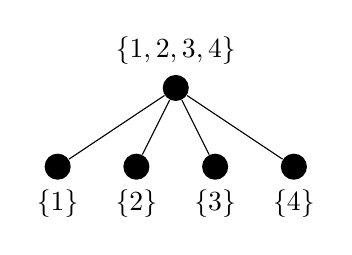
\begin{tikzpicture}[level distance = 10mm,sibling distance=10mm]
					\tikzstyle{active}=[circle,fill=black]
					\node [active,label={above:{$\{1,2,3,4\}$}}]  {}
					child {node [active,label=below:{$\{1\}$}]  {}}
					child {node [active,label=below:{$\{2\}$}]  {}}
					child {node [active,label=below:{$\{3\}$}]  {}}
					child {node [active,label=below:{$\{4\}$}]  {}};
					\end{tikzpicture}
					\caption{A trivial tree.}
					\label{fig:trivialTree}
				\end{subfigure}
				\begin{subfigure}[b]{.32\textwidth}
					\centering
					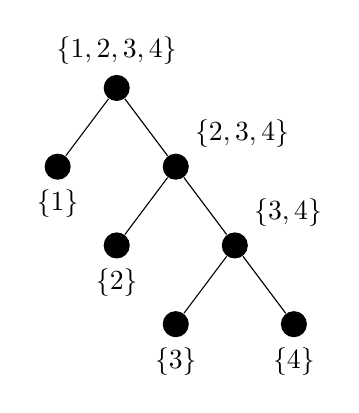
\begin{tikzpicture}[level distance = 10mm,sibling distance=10mm]
					\tikzstyle{active}=[circle,fill=black]
					\tikzstyle{level 1}=[sibling distance=15mm]
					\tikzstyle{level 2}=[sibling distance=15mm]
					\tikzstyle{level 3}=[sibling distance=15mm]
					\node [active,label={above:{$\{1,2,3,4\}$}}]  {}
					child {node [active,label=below:{$\{1\}$}]  {}
					}
					child {node [active,label=above right:{$\{2,3,4\}$}] {}
						child {node [active,label=below:{$\{2\}$}] {}}
						child {node [active,label=above right:{$\{3,4\}$}] {}
							child {node [active,label=below:{$\{3\}$}] {}}
							child {node [active,label=below:{$\{4\}$}] {}}
						}
					};
					\end{tikzpicture}
					\caption{A linear binary tree.}
					\label{fig:linearTree}
				\end{subfigure}
				\begin{subfigure}[b]{.32\textwidth}
					\centering
					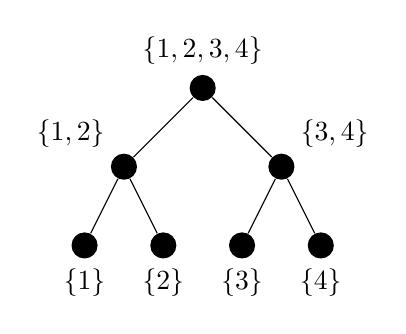
\begin{tikzpicture}[level distance = 10mm,sibling distance=10mm]
					\tikzstyle{active}=[circle,fill=black]
					\tikzstyle{level 1}=[sibling distance=20mm]
					\tikzstyle{level 2}=[sibling distance=10mm]
					\node [active,label={above:{$\{1,2,3,4\}$}}]  {}
					child {node [active,label=above left:{$\{1,2\}$}]  {}
						child {node [active,label=below:{$\{1\}$}] {}}
						child {node [active,label=below:{$\{2\}$}] {}}
					}
					child {node [active,label=above right:{$\{3,4\}$}] {}
						child {node [active,label=below:{$\{3\}$}] {}}
						child {node [active,label=below:{$\{4\}$}] {}}
					};
					\end{tikzpicture}
					\caption{A balanced binary tree.}
					\label{fig:balancedTree}
				\end{subfigure}
				\caption{Examples of dimension partition trees over $D=\{1,\hdots,4\}$.}
				\label{fig:treeExamples}
			\end{figure}
		
			\paragraph{Creating a \cmd{DimensionTree}.}
				A \cmd{DimensionTree} is characterized by its adjacency matrix and the dimension associated with each leaf node: \cmd{T = tensap.DimensionTree(dims, adjacency_matrix)}.
				The adjacency matrix of a dimension tree $T$ can be accessed with \cmd{T.adjacency_matrix}. 
				The dimension associated with each leaf node can be accessed with \cmd{T.dim2ind}. 
				
				Denoting by \cmd{order} the number of leaf nodes, it is possible to create
				\begin{itemize}
					\item a trivial tree with \cmd{tensap.DimensionTree.trivial(order)} (Figure \ref{fig:trivialTree}),
					\item a linear tree with \cmd{tensap.DimensionTree.linear(order)} (Figure \ref{fig:linearTree}),
					\item a balanced tree with \cmd{tensap.DimensionTree.balanced(order)}(Figure \ref{fig:balancedTree}),
					\item a random tree with \cmd{tensap.DimensionTree.random(order, arity)}, with \cmd{arity} the arity of the tree, equal to the maximum number of children per node (randomly selected in an interval if provided).
				\end{itemize}
				Finally, a dimension tree can be created by extracting a sub-tree from an existing tree $T$ with \cmd{T.sub_dimension_tree(root)} where \cmd{root} is the node in $T$ that will become the root node of the extracted tree.
			
			\paragraph{Displaying a \cmd{DimensionTree}.}
				A \cmd{DimensionTree} can be displayed with the command \cmd{T.plot()}.
				The dimension associated with each leaf node can be plotted on the tree with \cmd{T.plot_dims()}.
				Finally, the tree can be plotted with some quantity displayed at each node with \cmd{T.plot_with_labels_at_nodes(labels)}.
				
			\paragraph{Accessing properties of the tree.}	
				The number of nodes of a dimension tree $T$ is given by \cmd{T.nb_nodes}.
				
				The parent of $\alpha$, denoted by $P(\alpha)$, can be obtained with \cmd{T.parent(alpha)}, and its ascendants $A(\alpha)$ and descendants $D(\alpha)$ by \cmd{T.ascendants(alpha)} and \cmd{T.descendants(alpha)}, respectively.
				The children of $\alpha$ are given by \cmd{T.children(alpha)}.
				The command \cmd{T.child_number(alpha)} returns $i^\gamma_\alpha$, for $\alpha \in T \setminus \{D\}$ and $\gamma = P(\alpha)$, which is such that $\alpha$ is the $i^\gamma_\alpha$-th child of $\gamma$.
				For instance, in the tree of Figure \ref{fig:linearTree}, the node $\alpha = \{3,4\}$ is the second child of $\gamma = \{2,3,4\}$.
				
				The level of a node $\alpha$ is denoted by $\level(\alpha)$. 
				The levels are defined such that $\level(D) = 0$ and $\level(\beta) = \level(\alpha) + 1$ for $\beta \in S(\alpha)$. 
				The nodes of $T$ with level $l$ are returned by \cmd{T.nodes_with_level(l)}.
				
				The leaf nodes $\alpha \in \Lc(T)$ 
				 are such that \cmd{T.is_leaf[alpha-1]} is \cmd{True}.

		\subsubsection{\cmd{TreeBasedTensor}}
			Given a dimension tree $T$, a \cmd{TreeBasedTensor} \cmd{X} is a tensor in \emph{tree-based format} (see \cite{Falco2018SEMA,hackbusch2019tensor}). It represents an order $d$ tensor $X \in \Rbb^{N_1 \times \cdots \times N_d}$ in the set of tensors with $\alpha$-ranks bounded by some integer $r_\alpha$, $\alpha \in T$. Such a tensor admits a representation 
			\begin{equation*}
				X_{i_1, \hdots, i_d} = \sum_{\substack{1 \leq k_\beta \leq r_\beta \\�\beta \in T\setminus \{D\}}} \prod_{\alpha \in T\setminus \Lc(T)} C^\alpha_{(k_\beta)_{\beta \in S(\alpha)},k_\alpha} \prod_{\alpha \in \Lc(T)} C^{\alpha}_{i_\alpha,k_\alpha},
			\end{equation*}
			with $C^\alpha$, $\alpha \in T$, some tensors that parameterize the representation of $X$. 			
			When $T$ is a binary tree, the corresponding format is the so-called hierarchical Tucker (HT) format. The particular case of a linear binary tree is the tensor train Tucker format. 
			\\
			
			The \emph{Tucker format} corresponds to a trivial tree $T=\{\{1\},\hdots,\{d\},\{1,\hdots,d\}\} $ and admits the representation
			$$
			X_{i_1, \hdots, i_d} = \sum_{k_1=1}^{r_1} \hdots \sum_{k_d=1}^{r_d} C^{1,\hdots,d}_{k_1,\hdots,k_d} C^{1}_{i_1,k_1} \hdots C^{d}_{i_d,k_d}.
			$$
			
			A \emph{degenerate tree-based format} is defined as the set of tensors with $\alpha$-ranks bounded by some integer $r_\alpha$, for all $\alpha$ in a subset $A$ of $T$. The set $A$ corresponds to active nodes, which should contain all interior nodes $T\setminus\Lc(T)$. 
			A \cmd{TreeBasedTensor} \cmd{X} with active nodes $A$ admits a representation. 
						\begin{equation*}
				X_{i_1, \hdots, i_d} = \sum_{\substack{1 \leq k_\beta \leq r_\beta \\�\beta \in A \setminus \{D\}}} \prod_{\alpha \in A\setminus \Lc(T)} C^\alpha_{(k_\beta)_{\beta \in S(\alpha)},k_\alpha} \prod_{\alpha \in \Lc(T) \cap A} C^{\alpha}_{i_\alpha,k_\alpha},
			\end{equation*}
			with $C^\alpha$, $\alpha \in A$, some tensors that parameterize the representation of $X$. 
				
	The \emph{tensor train format} is a degenerate tree-based format  with a linear tree $T$ and all leaf nodes inactive except the first one, that means $A = \{\{1\},\{1,2\}, \hdots, \{1,\hdots,d\}\}$.  A tensor $X$ in tensor train format admits a representation
				$$
				X_{i_1,\hdots,i_d} = \sum_{k_1=1}^{r_1} \hdots \sum_{k_{d-1}=1}^{r_{d-1}} C^1_{1,i_1,k_1} C^2_{k_1,i_2,k_2} \hdots C^{d-1}_{k_{d-2},i_{d-1},k_{d-1}} C^d_{k_{d-1},i_d,1}
				$$
				with tensor $C^\nu$ and rank $r_\nu$ associated with the node $\alpha = \{1,\hdots,\nu\}$.
					 \\	
								
					 For a more detailed presentation of {tree-based formats} (possibly degenerate) and more examples, see \cite[Section 4]{nouy:2017hopca}.\\
					 
					 					 
					 			If the rank $r_D$ associated with the root node is different from $1$, a \cmd{TreeBasedTensor} \cmd{X} represents a tensor of order $d+1$ with entries $X_{i_1,\hdots,i_d,k_D}$, $1\le k_D \le r_D$. I can be used to defined vector-valued functional tensors (see \Cref{sec:FunctionTensor}). 
								
								
							
			
			\paragraph{Creating a \cmd{TreeBasedTensor}.\\}
				
				A \cmd{TreeBasedTensor} is created with the command \cmd{X = tensap.TreeBasedTensor(C, T)}, with \cmd{C} the list of \cmd{FullTensor} objects representing the $C^\alpha$, $\alpha \in T$, and \cmd{T} a \cmd{DimensionTree}. If some entries of the list \cmd{C} corresponding to leaf nodes are empty, it creates a degenerate tensor format, with $T\setminus A$ corresponding to the empty entries of \cmd{C}. 
\\

					It is possible to create a \cmd{TreeBasedTensor} �in tensor-train format with the command \cmd{tensap.TreeBasedTensor.tensor_train(C)}, with \cmd{C} a list containing the tensors $C^1,\hdots,C^d$.
\\

								Given a \cmd{DimensionTree} \cmd{T}, it is also possible to generate a \cmd{TreeBasedTensor} with entries
					\begin{itemize}
						\item equal to 0 with \cmd{tensap.TreeBasedTensor.zeros(T, r, s, I)},
						\item equal to 1 with \cmd{tensap.TreeBasedTensor.ones(T, r, s, I)},
						\item drawn randomly according to the uniform distribution on $[0, 1]$ with \cmd{tensap.TreeBasedTensor.rand(T, r, s, I)},
						\item drawn randomly according to the standard gaussian distribution with \cmd{tensap.TreeBasedTensor.randn(T, r, s, I)},
						\item generated using a provided \cmd{generator} with \cmd{tensap.TreeBasedTensor.create} \cmd{(generator, T, r, s, I)},
					\end{itemize}
					where \cmd{r} is a list containing the $\alpha$-ranks, $\alpha \in T$, or \cmd{'random'}, \cmd{s} is a list containing the sizes $N_1, \hdots, N_d$, or \cmd{'random'}, and \cmd{I} is a list of booleans indicating if the node $\alpha$ is active, $\alpha \in T$, or \cmd{'random'}.
				
			\paragraph{Storage complexity. }
			 						The storage complexity of \cmd{X} is given by $\cmd{X.size = X.storage()}$ and returns the number of entries in tensors $C^\alpha$, $\alpha\in A$.
				\\
					The storage complexity of \cmd{X} taking into account the sparsity in the $C^\alpha$, $\alpha \in T$, is given by \cmd{X.sparse_storage()}. It returns the number of non-zero entries  in tensors $C^\alpha$, $\alpha\in A$.\\
					The storage complexity of \cmd{X} taking into account the sparsity only in the leaf nodes is given by \cmd{X.sparse_leaves_storage()}.
			\paragraph{Displaying a \cmd{TreeBasedTensor}.}
				A graphical representation of a \cmd{TreeBasedTensor} \cmd{X} can be obtained with the command \cmd{X.plot()}.
				Labels can be added to the nodes of the tree, as well as a title, with \cmd{X.plot(labels, title)}.
			
			\paragraph{Converting a \cmd{TreeBasedTensor} to a \cmd{FullTensor}.}
				A \cmd{TreeBasedTensor} \cmd{X} can be converted to a \cmd{FullTensor} (introduced in Section \ref{sec:FullTensor}) with the command \cmd{X.full()}.

	\paragraph{Converting a \cmd{FullTensor} to a \cmd{TreeBasedTensor}.}
		A \cmd{FullTensor} \cmd{X} can be converted to a \cmd{TreeBasedTensor} with the command \cmd{X.tree_based_tensor()}.
		The associated dimension tree is a trivial tree with active nodes.
	
	
			\paragraph{Accessing the entries of a \cmd{TreeBasedTensor}.}
				The entries of the tensor \cmd{X} can be accessed with the method \cmd{eval_at_indices}: \cmd{X.eval_at_indices(ind)} returns the entries of $X$ indexed by the list \cmd{ind} containing the indices to access in each dimension.
				
A sub-tensor can be extracted from \cmd{X} with the method \cmd{sub_tensor} (see \Cref{sec:subtensor})

				
				For a tensor $X \in \Rbb^{N, \hdots, N}$, the command \cmd{X.eval_diag()} returns the diagonal $X_{i, \hdots, i}$, $i = 1, \hdots, N$, of the tensor. 
				The method \cmd{eval_diag} can also be used to evaluate the diagonal in some dimensions \cmd{dims} of the tensor with \cmd{X.eval_diag(dims)}.
				
			\paragraph{Obtaining an orthonormal representation of a \cmd{TreeBasedTensor}.}
				The command \cmd{X.orth()} returns a representation of \cmd{X} where all the core tensors except the root core represent orthonormal bases of principal subspaces.
				
				The command \cmd{X.orth_at_node(alpha)} returns a representation of \cmd{X} where all the core tensors except the one of node $\alpha$ represent orthonormal bases of principal subspaces.
				The core tensor $C^\alpha$ of the node $\alpha$ is such that the tensor writes 
				\begin{equation*}
					X_{i_\alpha, i_{\alpha^c}} = \sum_{k} \sum_{l} C^\alpha_{k,l} u_l(i_\alpha) w_k(i_{\alpha^c}),
				\end{equation*} 
				where the $u_l$ are orthonormal tensors and the $w_k$ are orthonormal tensors.
				This orthonormality of the representation can be checked by computing the Gram matrices of the bases of minimal subspaces associated with the nodes of the tree with \cmd{X.gramians()}.
					
			\paragraph{Modifying the tree structure of a \cmd{TreeBasedTensor}.}
				It is possible to modify the tree of a \cmd{TreeBasedTensor} \cmd{X} by permuting two of its nodes $\alpha$ and $\beta$ given a relative tolerance \cmd{tol} with \cmd{X.permute_nodes([alpha, beta], tol)}.
				
				The leaves of the tree can also be permuted with the command \cmd{X.permute_leaves(perm, tol)}, where \cmd{perm} is a permutation of $(1, \hdots, d)$.
				
				The method \cmd{optimize_dimension_tree} tries random permutations of nodes to minimize the storage complexity of a tree-based tensor $X$: \cmd{X.optimize_dimension_tree(tol, n)} tries $n$ random permutations and returns a \cmd{TreeBasedTensor} \cmd{Y} which is such that \cmd{Y.storage()} is less or equal than \cmd{X.storage()}.
				The nodes to permute are drawn according to probability measures favoring high decreases of the ranks while maintaining a permutation cost as low as possible (see \cite[Section 4.2.1]{grelier2019learning}).
			
				The similar method \cmd{optimize_leaves_permutations} focuses on the permutation of the leaf nodes to try to reduce the storage complexity of a \cmd{TreeBasedTensor}.
				
			\paragraph{Computing the Frobenius norm of a \cmd{TreeBasedTensor}.}
				The command \cmd{X.norm()} returns the Frobenius norm of $X$.
								
			\paragraph{Computing the $\alpha$-singular values of a \cmd{TreeBasedTensor}.}
				For all $\alpha \in T$, the $\alpha$-singular values of $X$ can be obtained with \cmd{X.singular_values()}.
				
				The method \cmd{rank} uses the method \cmd{singular_values} to compute the $\alpha$-ranks, $\alpha \in T$, of a \cmd{TreeBasedTensor}.
				
			\paragraph{Computing the derivative of \cmd{TreeBasedTensor} with respect to one of its parameters.}
				For an order-$d$ tree-based tensor \cmd{X} in $\Rbb^{N \times \cdots \times N}$, \cmd{X.parameter_gradient_eval_diag(alpha)}, for $\alpha \in T$, returns the derivative
				\begin{equation*}
					\left.\frac{\partial X_{i_1, \hdots, i_d}}{\partial C^\alpha}\right|_{i_1=\cdots=i_d=i}, \; i = 1, \hdots, N.
				\end{equation*}
				
				The method \cmd{parameter_gradient_eval_diag} is used in the statistical learning algorithms presented in Section \ref{sec:TensorLearning}.
				
			\paragraph{Performing operations with \cmd{TreeBasedTensor}.}	
			Some operations between tensors  are implemented for \cmd{TreeBasedTensor} (see \Cref{sec:operations-fulltensor} for a detailed description of the operations): the Kronecker product with \cmd{kron}, the contraction with matrices or vectors with \cmd{tensor_matrix_product} or \cmd{tensor_vector_product} respectively, the evaluation of the diagonal of a contraction with matrices with \cmd{tensor_matrix_product_eval_diag}, the dot product with \cmd{dot}. 
				
			\cmd{Z = X.tensor_matrix_product(M)}
			\cmd{tensor_vector_product}
			\cmd{tensor_matrix_product_eval_diag}
			\cmd{X.kron(Y)}
			\cmd{X.dot(Y)}
				


	\subsection{Tensor truncation with \cmd{Truncator}}
		The object \cmd{Truncator} embeds several methods of truncation of tensors in different formats.		
		Given a tolerance \cmd{tol} and a maximum rank or tuple of ranks \cmd{r}, a \cmd{Truncator} object can be created with \cmd{t = tensap.Truncator(tol, r)}.
		The thresholding type (\cmd{'hard'} or \cmd{'soft'}) can also be specified as a third argument.
		
		For examples of use, see the tutorial file \texttt{tutorials\textbackslash tensor\_algebra\textbackslash tutorial\_tensor\_truncation.py}.


		\paragraph{Truncation.}
			The generic method \cmd{truncate} calls one of the methods presented below, based on the type and order of its input, to obtain a truncation of the provided tensor satisfying the relative prevision and maximal rank requirements.
			
			For an order $2$ tensor, the method \cmd{svd} is called. 
			For a tensor of order greater than $2$, the method \cmd{hosvd} is called for a \cmd{FullTensor}, and \cmd{hsvd} for a \cmd{TreeBasedTensor}.
		
		\paragraph{Truncated singular value decomposition.}
			The method \cmd{svd} computes the truncated singular value decomposition of an order $2$ tensor.
			The input tensor can be a \cmd{numpy.ndarray}, a \cmd{tensorflow.Tensor}, a \cmd{FullTensor} or a \cmd{CanonicalTensor}, in which case the method \cmd{trunc_svd} is called, or a \cmd{TreeBasedTensor}, in which case the method \cmd{hsvd} is called.
			
			The method \cmd{trunc_svd} computes the truncated singular value decomposition of a matrix, with a given relative precision in Schatten $p$-norm (with a specified value for $p$) and given maximal rank.
			The returned truncation is a \cmd{CanonicalTensor}.
			
		\paragraph{Truncated higher-order singular value decomposition.}
			A truncated higher-order singular value decomposition of a \cmd{numpy.ndarray}, a \cmd{FullTensor} or a \cmd{TreeBasedTensor} can be computed with the method \cmd{hosvd}.
			The output is either a \cmd{CanonicalTensor} for an order $2$ tensor, or a \cmd{TreeBasedTensor} with a trivial tree for a tensor of order greater than $2$.
		
		\paragraph{Truncation in tree-based tensor format.}
			The method \cmd{hsvd} computes, given a \cmd{TreeBasedTensor} or a \cmd{FullTensor} with a tree and a set of active nodes, a truncation in tree-based tensor format.
			
			\paragraph{Truncation in tensor train format.}
			The method \cmd{ttsvd}, given a \cmd{FullTensor}, calls the method \cmd{hsvd} with a linear tree and all the leaf nodes inactive except the first one, resulting in a truncation in tensor-train format.
		
\section{Measures, bases and functions}
	\subsection{\cmd{RandomVariable}}
		A random variable $X$ can be created by calling its name: for instance, \cmd{X = tensap.UniformRandomVariable(a, b)} creates a random variable with a uniform distribution on the interval $[a, b]$.
		The random variables currently implemented in tensap are:
		\begin{itemize}
			\item \cmd{tensap.DiscreteRandomVariable(v, p)}: a random variable with discrete values $v$ and associated probabilities $p$,
			\item \cmd{tensap.UniformRandomVariable(a, b)}: a uniform random variable on $[a, b]$,
			\item \cmd{tensap.NormalRandomVariable(m, s)}: a normal random variable with mean $m$ and standard deviation $s$,
			\item \cmd{tensap.EmpiricalRandomVariable(S)}: a random variable created from a sample $S$ using kernel density estimation with Scott's rule of thumb to determine the bandwidth.
		\end{itemize}
		A new random variable can easily be implemented in tensap by making its class inheriting from \cmd{RandomVariable} and implementing the few methods necessary for its creation.
		
		Once a random variable $X$ is created, one can for instance generate $n$ random numbers according to its distribution with \cmd{X.random(n)}, create the orthonormal polynomials associated with its measure with \cmd{X.orthonormal_polynomials()} (as presented in Section \ref{sec:polynomials}), or evaluate its probability density function (\cmd{X.pdf(x)}), cumulative distribution function (\cmd{X.cdf(x)}) or inverse cumulative distribution function (\cmd{X.icdf(x)}).
			
	\subsection{\cmd{RandomVector}}
		A random vector $X$ if defined in tensap by a list of \cmd{RandomVariable} objects and a \cmd{Copula}, characterizing the dependencies between the random variables.
		Currently, only the independent copula \cmd{IndependentCopula} is implemented.
		
		Given a list of \cmd{RandomVariable} \cmd{random_variables} and a \cmd{Copula C}, a random vector can be created with \cmd{X = tensap.RandomVector(random_variables, copula=C)}.
		
		Once a random vector $X$ is created, one can for instance generate $n$ random numbers according to its distribution with \cmd{X.random(n)}, create the orthonormal polynomials associated with its measure with \cmd{X.orthonormal_polynomials()} (as presented in Section \ref{sec:polynomials}), or evaluate its probability density function (\cmd{X.pdf(x)}) or cumulative distribution function (\cmd{X.cdf(x)}).
			
	\subsection{\cmd{Polynomials}}
	\label{sec:polynomials}
		Families of univariate polynomials $(p_i)_{i\ge 0}$ are represented in tensap with classes inheriting from \cmd{UnivariatePolynomials}.
		The $i$-th polynomial $p_i$ represented by a \cmd{UnivariatePolynomials} object \cmd{P} can be evaluated with \cmd{P.polyval(x, i)}, as well as its first order derivative (\cmd{P.d_polyval(x, i)}) and its $n$-th order derivative (\cmd{P.dn_polyval(x, n, i)}).
		
		Given a measure $\mu$, the moments $\int  p_{i_1}(x)...p_{i_k}(x) d\mu(x)$ for $(i_1,...,i_k) \in \Nbb^{k}$ can be obtained with \cmd{P.moment(I, mu)}, with $\cmd{I}$ a $n$-by-$k$ array representing $n$ tuples $(i_1,...,i_k)$. \cmd{P.moment(I, X)} with $\cmd{X}$ a random variable considers for $\mu$ the probability distribution of $X$.
		
		
		\paragraph{\cmd{CanonicalPolynomials}.}
			The family of canonical polynomials is implemented in the class \cmd{CanonicalPolynomials}.
			It is such that its $i$-th polynomial is $p_i(x) = x^i$.
			
		\paragraph{\cmd{OrthonormalPolynomials}.}
			Orthonormal polynomials are families of polynomials $(p_i)_{i \geq 0}$ that satisfy 
			\begin{equation*}
				\int p_i(x) p_j(x) d\mu(x)= \delta_{ij}
			\end{equation*}
			with $\delta_{ij}$ the Kronecker delta, and with $\mu$ some measure. 
			
			In tensap, the orthonormal polynomials $p_i$, $i \geq 0$, are defined using the three-term recurrence relation 
			\begin{align*}
				&\tilde p_{-1}(x) = 0, \quad \tilde p_0(x) = 1, \\
				&\tilde p_{i+1}(x) = (x - a_i)\tilde p_{i}(x) - b_i \tilde p_{i-1}(x), \quad i \geq 0,\\
				&p_i(x) = \frac{\tilde p_i(x)}{n_i}, \quad i \geq 0
			\end{align*}
			with $a_i$ and $b_i$ the recurrence coefficients, and $n_i$ the norm of $\tilde p_i$, defined by
			\begin{equation*}
				a_i = \frac{\int \tilde p_i(x) x \tilde p_i(x) d\mu(x)}{\int p_i(x) \tilde p_i(x) d\mu(x)}, \quad 
				b_i = \frac{\tilde p_i(x) \tilde p_i(x) d\mu(x)}{\int \tilde p_{i-1}(x) \tilde p_{i-1}(x)  d\mu(x)}, \quad
				n_i = \sqrt{\int\tilde p_i(x) \tilde p_i(x) d\mu(x)}.
			\end{equation*}
			 	Implementing a new family of orthonormal polynomials in tensap is easy: one only needs to create a class with a method providing the recurrence coefficients $a_i$, $b_i$ and the norms $n_i$, $\forall i \geq 0$.
\\

\noindent			Are currently implemented in tensap:
			\begin{itemize}
				\item \cmd{DiscretePolynomials}: discrete polynomials orthonormal with respect to the measure of a \cmd{DiscreteRandomVariable};
				\item \cmd{LegendrePolynomials}: polynomials defined on $[-1,1]$ and orthonormal with respect to the uniform measure on $[-1,1]$ with density $\frac{1}{2}\mathbf{1}_{[-1,1]}(x)$;
				\item \cmd{HermitePolynomials}: polynomials defined on $\Rbb$ and orthonormal with respect to the standard gaussian measure with density  $\exp(-x^2/2)/\sqrt{2\pi}$;
				\item \cmd{EmpiricalPolynomials}: polynomials orthonormal with respect to the measure of an \cmd{EmpiricalRandomVariable}.
			\end{itemize}
If \cmd{mu} is a \cmd{LebesgueMeasure} on $[-1,1]$, \cmd{mu.orthonormal_polynomials()} returns a \cmd{LegendrePolynomials} with suitably normalized coefficients. If \cmd{mu} is a \cmd{LebesgueMeasure} on $[a,b]$ different from $[-1,1]$, \cmd{mu.orthonormal_polynomials()} returns a \cmd{ShiftedOrthonormalPolynomials}.
			\\
			
\noindent 		If $\cmd{X}$ is a \cmd{DiscreteRandomVariable}, a \cmd{UniformRandomVariable}, a \cmd{NormalRandomVariable}, or a \cmd{EmpiricalRandomVariable}, the corresponding family of orthonormal polynomials can be created with the command \cmd{X.orthonormal_polynomials()}. If $\cmd{X}$ does not correspond to a default measure but can be obtained as the push-forward measure of a default measure by an affine transformation  (e.g. a uniform measure on $[a,b] \neq [-1,1]$, or a gaussian measure with mean $a$ and standard deviation $\sigma$ with $(a,\sigma)\neq (0,1)$.), the returned object is a \cmd{ShiftedOrthonormalPolynomials}.
		
		
		
			
			
	\subsection{\cmd{FunctionalBasis}}
		Bases of functions can be implemented in tensap by inheriting from \cmd{FunctionalBasis}.	
		The basis functions of a \cmd{FunctionalBasis} object \cmd{H} can be evaluated with \cmd{H.eval(x)}, as well as their $i$-th order derivative with \cmd{H.eval_derivative(i, x)}.
		\\
		
		We present below some specific bases implemented in tensap. 
		New bases can easily be implemented by making their class inherit from \cmd{FunctionalBasis}.
		
		\paragraph{\cmd{PolynomialFunctionalBasis}.}
			The command \cmd{tensap.PolynomialFunctionalBasis} \cmd{(basis, indices)}, with \cmd{basis} a \cmd{UnivariatePolynomials} and \cmd{indices} a list, returns the basis of polynomials $(p_i)_{i \in I}$ with $I$ given by \cmd{indices}.
		
		\paragraph{\cmd{UserDefinedFunctionalBasis}.}
			Given a list of functions \cmd{fun}, taking each as inputs $d$ variables, and a \cmd{Measure mu}, the command \cmd{tensap.UserDefinedFunctionalBases(fun, mu, d)} returns a basis whose functions are the ones given in \cmd{fun}, with a domain equipped with the measure $mu$.
		
		\paragraph{\cmd{FullTensorProductFunctionalBasis}.}
			A \cmd{FullTensorProductFunctionalBasis} object represents a basis of multivariate functions $\{\phi^1_{i_1}(x_1) \cdots \phi^d_{i_d}(x_d)\}_{i_1 \in I^1, \hdots, i_d \in I^d}$.
			It is obtained with the command \cmd{tensap.FullTensorProductFunctionalBasis(bases)}, where \cmd{bases} is a list of \cmd{FunctionalBasis} or a \cmd{FunctionalBases}, containing the different bases $\{\phi^\nu_{i_\nu}\}_{i_\nu \in I^\nu}$, $\nu = 1, \hdots, d$.
		
		\paragraph{\cmd{SparseTensorProductFunctionalBasis}.}
			A \cmd{SparseTensorProductFunctionalBasis} object represents a basis of multivariate  functions $\{\phi^1_{i_1}(x_1) \cdots \phi^d_{i_d}(x_d)\}_{(i_1, \hdots, i_d) \in \Lambda}$, with $\Lambda \subset I^1 \times \cdots \times I^d$ a set of multi-indices.
			It is obtained with the command \cmd{tensap.SparseTensorProductFunctionalBasis(bases, indices)}, where \cmd{bases} is a list of \cmd{FunctionalBasis} or a \cmd{FunctionalBases}, containing the different bases $\{\phi^\nu_{i_\nu}\}_{i_\nu \in I^\nu}$, $\nu = 1, \hdots, d$, and \cmd{indices} is a \cmd{MultiIndices} representing the set of multi-indices $\Lambda$.
		
	\subsection{\cmd{FunctionalBases}}
		The command \cmd{tensap.FunctionalBases(bases)}, with \cmd{bases} a list of \cmd{FunctionalBasis}, returns an object representing a collections of bases.
		To obtain a collection of $d$ identical bases, one can use \cmd{tensap.FunctionalBases.duplicate(basis, d)}.
		
		Similarly to \cmd{FunctionalBasis}, the basis functions of a \cmd{FunctionalBases} object \cmd{H} can be evaluated with \cmd{H.eval(x)}, as well as their $i$-th order derivative with \cmd{H.eval_derivative(i, x)}.
			
	
	\subsection{\cmd{FunctionalBasisArray}}
		Given a basis of functions $\{\phi_{i}\}_{i \in I}$, a \cmd{FunctionalBasisArray} object represents a function $f$ that writes
		\begin{equation*}
			f(x) = \sum_{i \in I} a_i \phi_i(x),
		\end{equation*}
		with some coefficients $a_i$, $i \in I$, and can be created with the command \cmd{f = tensap.FunctionalBasisArray(a, basis, shape)}, with \cmd{shape} the output shape of $f$.
		
		A \cmd{FunctionalBasisArray} is a \cmd{Function}. It can be evaluated with the command \cmd{f.eval(x)}, and one can obtain its derivatives with \cmd{f.eval_derivative(n, x)}.
		
	\subsection{\cmd{FunctionalTensor}}\label{sec:FunctionTensor}
		Given $d$ bases of functions $\{\phi^\nu_{i_\nu}\}_{i_\nu \in I^\nu}$, $\nu = 1, \hdots, d$, and a tensor $a \in \Rbb^{I^1 \times \cdots \times I^d}$, a \cmd{FunctionalTensor} object represents a function $f$ that writes
		\begin{equation*}
			f(x) = \sum_{i_1 \in I^1} \cdots \sum_{i_d \in I^d} a_{i_1, \hdots, i_d} \phi^1_{i_1}(x_1) \cdots \phi^d_{i_d}(x_d).
		\end{equation*}
		The tensor $a$ can be in different tensor formats (\cmd{FullTensor}, \cmd{TreeBasedTensor}, ...).
		
%If the tensor \cmd{a} is of order $d+1$,  the \cmd{FunctionalTensor} object represent a vector-valued function with components
%\begin{equation*}
%			f_k(x) = \sum_{i_1 \in I^1} \cdots \sum_{i_d \in I^d} a_{i_1, \hdots, i_d,k} \phi^1_{i_1}(x_1) \cdots \phi^d_{i_d}(x_d).
%		\end{equation*}
%	If \cmd{a} is a tree-based tensor, the number of components is the root rank $r_D$. 
		
	A \cmd{FunctionalTensor} is a \cmd{Function}. It can be evaluated with the command \cmd{f.eval(x)}, and one can obtain its derivatives with \cmd{f.eval_derivative(n, x)}.

	\subsection{\cmd{Tensorizer} and \cmd{TensorizedFunction}}
	For an introduction to tensorization of functions, see \cite{Ali2020ApproximationWTpartI,Ali2020ApproximationWTpartII}. 
	\\
	
		We consider functions defined on the interval $I = [0,1)$.
		For a given $b \in \{2,3,\hdots, \}$ and $d\in \Nbb$, an element $x \in I$ can be identified with the tuple $(i_1,\hdots,i_d,y)$, such that
		\begin{equation} \label{eq:tensorization}
			x = t_{b,d}(i_1,\hdots,i_d,y) = \sum_{k=1}^d i_kb^{-k} + b^{-d}y
		\end{equation}
		with $i_k \in I_b = \{0,\hdots,b-1\}$, $k = 1,\hdots,d$, and $y = b^d x - \lfloor b^d x \rfloor \in [0,1)$.
		The tuple $(i_1,\hdots,i_d)$ is the representation in base $b$ of $\lfloor b^d x \rfloor$.
		This defines a bijective map $t_{b,d}$ from $\{0,\hdots,b-1\}^{d} \times [0,1)$ to $[0,1)$. 
		
		 Such a mapping is represented in tensap by the object \cmd{Tensorizer}: \cmd{t = tensap.Tensorizer(b, d)}.
		For a given $x$ in $[0,1)$, on obtains the corresponding tuple $(i_1, ..., i_d,y)$ with the command \cmd{= t.map(x)}. For a given tuple $(i_1, ..., i_d,y)$, on obtains  the corresponding $x$ with \cmd{t.inverse_map([i_1, ..., i_d,y])}.
		
		This identification is generalized to functions of $D$ variables with \cmd{t = tensap.Tensorizer(b, d, D)}.
		
The map $t_{b,d}$ allows to define a tensorization map $T_{b,d}$, which associates to a univariate function $F$ defined on $[0,1)$ the multivariate function $f = F \circ t_{b,d}$ defined on $I_b^d \times I$,  such that 
		\begin{equation*}
			f(i_1,\hdots,i_d,y) = F(t_{b,d}(i_1,\hdots,i_d,y)).
		\end{equation*}
		Such a function is represented in tensap by a \cmd{TensorizedFunction}, and can be created with \cmd{f = tensap.TensorizedFunction(fun, t)}, with \cmd{fun} a \cmd{function} or \cmd{Function} and \cmd{t} a \cmd{Tensorizer}.
		The \cmd{TensorizedFunction} \cmd{f} is a function of $d+1$ variables that can be evaluated with \cmd{f.eval(x)}, with \cmd{x} a list or \cmd{numpy.ndarray} with $d+1$ columns.
\\

See the tutorial file \texttt{tutorials\textbackslash functions\textbackslash tutorial\_TensorizedFunction.py}.



\section{Tools}


\subsection{\cmd{MultiIndices}}

A multi-index is a tuple $(i_1,\hdots,i_d) \in \Nbb_0^d$. A set $I \subset \Nbb_0^d$ of multi-indices is represented with an object  
\cmd{MultiIndices}.

To create a multi-index set $I$, we use the command \cmd{tensap.MultiIndices(I)} with \cmd{I} a numpy array of size $\#I \times d$.

A product set $I = I_1 \times \hdots \times I_d$ can be obtained with \cmd{tensap.MultiIndices.product_set([I1,...,Id])}. 

The set of multi-indices 
$$
I = \{i  \in \Nbb_0^d : \Vert i \Vert_{\ell^p} \le m\}
$$
can be obtained with \cmd{tensap.MultiIndices.with_bounded_norm(d, p, m)}

The set of multi-indices 
$$
I = \{i  \in \Nbb_0^d : i_\nu \le m_\nu , 1\le \nu \le d\}
$$
can be obtained with \cmd{tensap.MultiIndices.bounded_by(d, p, m)}. If $m$ is of length $1$, it uses $m_\nu = m$ for all $\nu$.

For obtaining the margin or reduced margin of an multi-index set $I$, we can use 
%% LEARNING %%

For other operations of \cmd{MultiIndices}, see the tutorial file \texttt{tutorials\textbackslash tools\textbackslash tutorial\_MultiIndices.py}.

\subsection{\cmd{TensorGrid}, \cmd{FullTensorGrid} and \cmd{SparseTensorGrid}}

Tensor product grids or sparse grids are represented with classes \cmd{FullTensorGrid} and \cmd{SparseTensorGrid}, that inherit from \cmd{TensorGrid}.
\\

See the tutorial file \texttt{tutorials\textbackslash functions\textbackslash tutorial\_functions\_bases\_grids.py}.

\section{Learning}
	We present in this section some objects implemented in tensap for learning functions or tensors.
	
	\subsection{\cmd{(Functional)TensorPrincipalComponentAnalysis}}
		The objects \cmd{TensorPrincipalComponentAnalysis} (resp. \cmd{FunctionalTensorPrincipalComponentAnalysis}) implements approximation methods for  algebraic (resp. functional) tensors based on principal component analysis, using an adaptive sampling of the entries of the tensor (or the function). See \cite{nouy:2017hopca} for a description of the algorithms, and  					
		for examples of use, see the tutorial files \texttt{tutorials\textbackslash approximation\textbackslash tutorial\_TensorPrincipalComponentAnalysis.py} and \texttt{tutorials\textbackslash approximation\textbackslash tutorial\_FunctionalTensorPrincipalComponentAnalysis.py}.

		
		The difference between the two objects if that \cmd{TensorPrincipalComponentAnalysis}' methods take as first input a function returning components of the algebraic tensor to learn, whereas the methods of \cmd{FunctionalTensorPrincipalComponentAnalysis} take as first input the functional tensor to learn.
		\\
				
		Both objects are parameterized by the attributes:
		\begin{itemize}
			\item \cmd{pca_sampling_factor}: a factor to determine the number of samples $N$ for the estimation of the principal components (1 by default): if the precision is prescribed, $N = \cmd{pca_sampling_factor} \times N_\alpha$, if the rank is prescribed, $N = \cmd{pca_sampling_factor} \times t$;
			\item \cmd{pca_adaptive_sampling}: a boolean indicating if  adaptive sampling is used to determine the principal components with prescribed precision;
			\item \cmd{tol}: an array containing the prescribed relative precision; set \cmd{tol = inf} for prescribing the rank;
			\item \cmd{max_rank}: an array containing the maximum alpha-ranks (the length depends on the format). If \cmd{len(max_rank) == 1}, uses the same value for all alpha; setting \cmd{max_rank = inf} prescribes the precision.
		\end{itemize} 
		Furthermore, a \cmd{FunctionalTensorPrincipalComponentAnalysis} is parameterized by the attributes:
		\begin{itemize}
			\item \cmd{bases}: the functional bases used for the projection of the function;
			\item \cmd{grid}: the \cmd{FullTensorGrid} used for the projection of the function on the functional bases;
			\item \cmd{projection_type}: the type of projection, the default being 'interpolation'.
		\end{itemize}

\noindent Both objects implement four main methods:
		\begin{itemize}
			\item \cmd{hopca}: returns the set of $\{\nu\}$-principal components of an order $d$ tensor, for all $\nu \in \{1,\hdots,d\}$;
			\item \cmd{tucker_approximation}: returns an approximation of a tensor of order $d$ or a function of $d$ variables in Tucker format;
			\item \cmd{tree_based_approximation}: provided with a tree and a list of active nodes, returns an approximation of a tensor of order $d$ or a function of $d$ variables in tree-based tensor format;
			\item \cmd{tt_approximation}: returns an approximation of a tensor of order $d$ or a function of $d$ variables in tensor-train format. 
		\end{itemize}

	\subsection{\cmd{LossFunction}}
		In tensap, a loss function is an object inheriting from \cmd{LossFunction}.
		Given a function \cmd{fun} and a sample as a list used to evaluate the loss function, a \cmd{LossFunction} object $\ell$ can be evaluated with \cmd{l.eval(fun, sample)}.
		The risk associated with \cmd{fun} can be evaluated using the sample with \cmd{l.risk_estimation(fun, sample)}.
		Finally, the test error and relative test error (if defined) can be evaluated with \cmd{l.test_error(fun, sample)} and \cmd{l.relative_test_error(fun, sample)}, respectively.
	\\
	
	\noindent	Currently, three loss functions are implemented in tensap:
		\begin{itemize}
			\item \cmd{SquareLossFunction}: $\ell(g, (x, y)) = (y - g(x))^2$,  used for least-squares regression in supervised learning, to construct an approximation of a random variable $Y$ as a function of a random vector $X$ (a predictive model);
			\item \cmd{DensityL2LossFunction}: $\ell(g, x) = \|g\|^2 - 2g(x)$, used for least-squares density estimation, to approximate the distribution of a random variable $X$ from samples of $X$;
			\item \cmd{CustomLossFunction}: defined by the user as any function defining a loss. If the loss is defined using tensorflow operations, then the empirical risk can be minimized using tensorflow's automatic differentiation capability with a \cmd{LinearModelLearningCustomLoss} object, presented in the next section.
		\end{itemize}
	
	\subsection{\cmd{LinearModelLearning}}
		Objects inheriting from \cmd{LinearModelLearning} implement the empirical risk minimization associated with a linear model 
		that writes $$g(x) = \sum_{i \in I} a_i \phi_i(x),$$ with $\{\phi_i\}_{i \in I}$ a given basis (or a set of features) and $(a_i)_{i \in I}$ some coefficients, and a loss function, introduced in the previous section.
		
		In order to perform empirical risk minimization, a \cmd{LinearModelLearning} object \cmd{s} must be provided with a training sample in \cmd{s.training_sample}. In supervised learning, for the approximation of a random variable $Y$ as a function of $X$, the training sample is a list  \cmd{[x, y]}, with $\cmd{y}$ represents $n$ samples $\{y_k\}_{k=1}^n$ of $Y$ and  $x$ the $n$ corresponding samples $\{x_k\}_{k=1}^n$ of  $X$. In density estimation, the training sample is an array \cmd{x}  containing samples $\{x_k\}_{k=1}^n$ from the distribution to estimate.
		
		One must also provide a basis (in \cmd{s.basis}) or evaluations of the basis on the training set (in \cmd{s.basis_eval}, in which case the $x$ are not mandatory in \cmd{s.training_sample}). The latter option allows for providing  features $\phi_i(x_k)$ associated with samples $x^k$, without providing the feature maps $\phi_i$.  
		
		One can also provide the \cmd{LinearModelLearning} \cmd{s} with a test sample in \cmd{s.test_data} to compute a test error.
		\\
		
		Currently in tensap, three different \cmd{LinearModelLearning} objects are implemented:
		\begin{itemize}
			\item \cmd{LinearModelLearningSquareLoss}, to minimize the risk associated with a  \cmd{SquareLossFunction};
			\item \cmd{LinearModelLearningDensityL2}, to minimize the risk associated with a  \cmd{DensityL2LossFunction};
			\item \cmd{LinearModelLearningCustomLoss}, to minimize the risk associated with a  \cmd{CustomLossFunction}.
		\end{itemize}
	
		\paragraph{\cmd{LinearModelLearningSquareLoss}.}
			A \cmd{LinearModelLearningSquareLoss} object \cmd{s} implements three ways of solving the empirical risk minimization associated with a \cmd{SquareLossFunction}:
			\begin{itemize}
				\item by default, \cmd{s.solve()} solves the ordinary least-squares problem
				\begin{equation*}
					\min_{(a_i)_{i \in I}} \frac 1 n \sum_{k=1}^n (y_k - \sum_{i \in I} a_i \phi_i(x_k))^2;
				\end{equation*}
				\item with the attribute \cmd{s.regularization = True}, \cmd{s.solve()} solves the regularized problem
				\begin{equation*}
					\min_{(a_i)_{i \in I}} \frac 1 n \sum_{k=1}^n (y_k - \sum_{i \in I} a_i \phi_i(x_k))^2 + \lambda \|a\|_p
				\end{equation*}
				with $\lambda$ a regularization hyper-parameter, selected with a cross-validation estimate of the error and $p$ specified by \cmd{s.regularization_type} which can be \cmd{'l0'} ($p = 0$), \cmd{'l1'} ($p = 1$) or \cmd{'l2'} ($p = 2$);
				\item let us suppose that we have a collection of candidate sparsity patterns $K_\lambda$, $\lambda \in \Lambda$, for the parameter $a$: with the attribute \cmd{s.basis_adaptation = True}, \cmd{s.solve()} solves, for all $\lambda\in \Lambda$, the problem 
				\begin{equation*}
					\min_{(a_i)_{i \in I}} \frac 1 n \sum_{k=1}^n (y_k - \sum_{i \in I} a_i \phi_i(x_k))^2 \quad \text{subject to } \mathrm{support}(a) \subset K_\lambda,
				\end{equation*}
				where $\mathrm{support}(a) = \{ k \in K : a_k \neq 0 \}$, and selects the optimal sparsity pattern using a cross-validation estimate of the error.
			\end{itemize}
		
		\paragraph{\cmd{LinearModelLearningDensityL2}.}
			A \cmd{LinearModelLearningDensityL2} object \cmd{s} implements three ways of solving the empirical risk minimization associated with a \cmd{DensityL2LossFunction}:
			\begin{itemize}
				\item by default, \cmd{s.solve()} solves the minimization problem
				\begin{equation*}
					\min_{(a_i)_{i \in I}} \| \sum_{i \in I} a_i \phi_i \|_{L^2}^2 - \frac 2 n \sum_{k=1}^n \sum_{i \in I} a_i \phi_i(x_k);
				\end{equation*}
				\item with the attribute \cmd{s.regularization = True}, \cmd{s.solve()} solves the constrained problem
				\begin{equation*}
					\min_{(a_i)_{i \in I}} \|\sum_{i \in I} a_i \phi_i \|_{L^2}^2 - \frac 2 n \sum_{k=1}^n \sum_{i \in I} a_i \phi_i(x_k) \quad \text{subject to } \mathrm{support}(a) \subset K_\lambda,
				\end{equation*}
				with $K_\lambda$, $\lambda \in \Lambda$, a sequence of sets of indices that introduce the coefficients solution of the minimization problem without regularization in decreasing order of magnitude. 
				The optimal sparsity pattern is determined using a cross-validation estimate of the error;
				\item let us suppose that we have a collection of candidate patterns $K_\lambda$, $\lambda \in \Lambda$, for the parameter $a$: with the attribute \cmd{s.basis_adaptation = True}, \cmd{s.solve()} solves, for all $\lambda\in \Lambda$, the problem 
				\begin{equation*}
					\min_{(a_i)_{i \in I}} \|\sum_{i \in I} a_i \phi_i \|^2 - \frac 2 n \sum_{k=1}^n \sum_{i \in I} a_i \phi_i(x_k) \quad \text{subject to } \mathrm{support}(a) \subset K_\lambda,
				\end{equation*}
				and selects the optimal sparsity pattern using a cross-validation estimate of the error.
			\end{itemize}
		
		\paragraph{\cmd{LinearModelLearningCustomLoss}.}
			A \cmd{LinearModelLearningCustomLoss} object \cmd{s} implements a way of solving the empirical risk minimization associated with a \cmd{CustomLossFunction} using tensorflow's automatic differentiation capabilities.
			
			By default, the optimizer used is keras' Adam algorithm, which is a ``stochastic gradient descent method that is based on adaptive estimation of first-order and second-order moments'' (per tensorflow's documentation).
			
			The algorithm requires a starting point, provided in \cmd{s.initial_guess}, and several options can be set: 
			\begin{itemize}
				\item \cmd{s.options['max_iter']} sets the maximum number of iterations used in the optimization  algorithm,
				\item \cmd{s.options['stagnation']} sets the stopping tolerance on the stagnation between two iterates,
				\item for the Adam algorithm (and other minimization algorithms provided by tensorflow/keras), the learning rate can be provided in \cmd{s.optimizer.learning_rate}.
			\end{itemize}
	
	\subsection{\cmd{TensorLearning}}
	\label{sec:TensorLearning}
		The package tensap implements algorithms to perform statistical learning with canonical and tree-based tensor formats. See \cite{grelier:2018,grelier2019learning,2020arXiv200701165M} for a detailed presentation of algorithms and related theory.
		
		For examples, see the tutorial files  \texttt{tutorials\textbackslash approximation\textbackslash tutorial\_tensor\_learning\_CanonicalTensorLearning.py}, \texttt{tutorials\textbackslash approximation\textbackslash tutorial\_tensor\_learning\_TreeBasedTensorLearning.py},  \texttt{tutorials\textbackslash approximation\textbackslash tutorial\_tensor\_learning\_TreeBasedTensorDensityLearning.py}, \texttt{tutorials\textbackslash approximation\textbackslash tutorial\_tensor\_learning\_tensorized\_function\_learning.py}.

		
		These algorithms are implemented in the core object \cmd{TensorLearning}, common to all the tensor formats, so that implementing such a learning algorithm for a new tensor format is simple.
		In tensap are currently implemented \cmd{CanonicalTensorLearning} for the learning in canonical tensor format and \cmd{TreeBasedTensorLearning} for the learning in tree-based tensor format.
		
		Two algorithms are proposed: the standard one, which minimizes an empirical risk over the set of tensors in a given format thanks to an alternating minimization over the parameters of the tensors, and the adaptive one, which returns a sequence of empirical risk minimizers with adapted rank (for the canonical and tree-based tensor formats) and adapted tree (for the tree-based tensor format).
		
		In order to perform empirical risk minimization, a \cmd{TensorLearning} object \cmd{s} must be provided with a training sample in \cmd{s.training_sample}.  In supervised learning, for the approximation of a random variable $Y$ as a function of $X$, the training sample is a list  \cmd{[x, y]}, with $\cmd{y}$ represents $n$ samples $\{y_k\}_{k=1}^n$ of $Y$ and  $x$ the $n$ corresponding samples $\{x_k = (x_{k,1},\hdots,x_{k,d})\}_{k=1}^n$ of  $X$. In density estimation, the training sample is an array \cmd{x}  containing samples $\{x_k= (x_{k,1},\hdots,x_{k,d})\}_{k=1}^n$ from the distribution to estimate.

	
		
		One must also provide bases (in \cmd{s.bases}) or evaluations of the bases on the training set (in \cmd{s.bases_eval}, in which case the $x$ are not mandatory in \cmd{s.training_sample}). The latter option allows for providing features $\phi^\nu_i(x_{\nu,k})$, $1\le \nu\le d$, associated with samples $x_k = (x_{k,1},\hdots,x_{k,d})$, without providing the feature maps $\phi^\nu_i$.  

		
		One can also provide the \cmd{TensorLearning} \cmd{s} with a test sample in \cmd{s.test_data} to compute a test error.
		
		\paragraph{Rank adaptation.} (See \cite[Section 4.1]{grelier:2018})
			The rank adaptation is enabled by setting \cmd{s.rank_adaptation} to \cmd{True}.
			
			For tensors in canonical format, the algorithm returns a sequence of rank-$r$ approximations, with $r = 1, \hdots, r_{\text{max}}$, $r_{\text{max}}$ being given by \cmd{s.rank_adaptation_options} \cmd{['max_iterations']}.
			
			For tensors in tree-based format,  the algorithm returns a sequence of tensors with non-decreasing tree-based rank, obtained by increasing, at each iterations, the ranks associated with a subset of nodes of the tree $T$.
			The number of nodes in this subset is influenced by a parameter \cmd{s.rank_adaptation_options['theta']} in $[0, 1]$, which is such that the larger it is, the more ranks are increased at each iteration. 
			The default value of $0.8$. 
			
		\paragraph{Tree adaptation.} (See \cite[Section 4.2]{grelier:2018})
			For tree-based tensor formats, the tree can be adapted at each iteration using the algorithm mentioned in Section \ref{sec:TreeBasedTensor}, by setting \cmd{s.tree_adaptation} to \cmd{True}.
			The tolerance for the tree adaptation is provided by \cmd{s.tree_adaptation_options['tolerance']} and the maximal number of tried trees by \cmd{s.tree_adaptation_options['max_iterations']}.
			
		\paragraph{Model selection.} (See \cite{2020arXiv200701165M})
			At the end of the adaptive procedure, a model can be selected by setting \cmd{s.model_selection} to \cmd{True}, using either a test error (specified by \cmd{s.model_selection_options['type'] = 'test_error'}) or a cross-validation estimate of the error (specified by \cmd{s.model_selection_options['type'] = 'cv_error'}).
	
	\subsection{Example: character classification in tree-based tensor format.}
			We present below a part of the tutorial file \texttt{tutorial\textbackslash tensor\textbackslash learning\textbackslash digits\textbackslash recognition.py} shipped with the package tensap.
			Its aim is to create a classifier in tree-based tensor format, able to recognize hand written digits from $0$ to $9$.
			
			The output of the algorithm is displayed below the Python script, as well as in Figure \ref{fig:classification_results}, which shows the confusion matrix on the test sample as well as a visual comparison on some test samples.
			We see that, using a training sample of size $1617$, it returns a classifier that obtains a score of $98.89\%$ of correct classification on a test sample of size $180$.
		
\bigskip
\begin{lstlisting}[language=Python, showstringspaces=false, title=Tutorial file tutorial\_tensor\_learning\_digits\_recognition.py]
from sklearn import datasets, metrics
import random
import numpy as np
import tensorflow as tf
import time
import matplotlib.pyplot as plt
import tensap

# %% Data import and preparation
DIGITS = datasets.load_digits()
DATA = DIGITS.images.reshape((len(DIGITS.images), -1))
DATA = DATA / np.max(DATA)  # Scaling of the data

# %% Patch reshape of the data: the patches are consecutive entries of the data
PS = [4, 4]  # Patch size
DATA = np.array([np.concatenate(
	[np.ravel(np.reshape(DATA[k, :], [8]*2)[PS[0]*i:PS[0]*i+PS[0],
											PS[1]*j:PS[1]*j+PS[1]]) for
	 i in range(int(8/PS[0])) for j in range(int(8/PS[1]))]) for
	k in range(DATA.shape[0])])
DIM = int(int(DATA.shape[1]/np.prod(PS)))

# %% Probability measure
print('Dimension %i' % DIM)
X = tensap.RandomVector(tensap.DiscreteRandomVariable(np.unique(DATA)), DIM)

# %% Training and test samples
P_TRAIN = 0.9  # Proportion of the sample used for the training

N = DATA.shape[0]
TRAIN = random.sample(range(N), int(np.round(P_TRAIN*N)))
TEST = np.setdiff1d(range(N), TRAIN)
X_TRAIN = DATA[TRAIN, :]
X_TEST = DATA[TEST, :]
Y_TRAIN = DIGITS.target[TRAIN]
Y_TEST = DIGITS.target[TEST]

# One hot encoding (vector-valued function)
Y_TRAIN = tf.one_hot(Y_TRAIN.astype(int), 10, dtype=tf.float64)
Y_TEST = tf.one_hot(Y_TEST.astype(int), 10, dtype=tf.float64)

# %% Approximation bases: 1, cos and sin for each pixel of the patch
FUN = [lambda x: np.ones((np.shape(x)[0], 1))]
for i in range(np.prod(PS)):
	FUN.append(lambda x, j=i: np.cos(np.pi / 2*x[:, j]))
	FUN.append(lambda x, j=i: np.sin(np.pi / 2*x[:, j]))

BASES = [tensap.UserDefinedFunctionalBasis(FUN, X.random_variables[0],
										   np.prod(PS)) for _ in range(DIM)]
BASES = tensap.FunctionalBases(BASES)

# %% Loss function: cross-entropy custom loss function
LOSS = tensap.CustomLossFunction(
		lambda y_true, y_pred: tf.nn.sigmoid_cross_entropy_with_logits(
			logits=y_pred, labels=y_true))


def error_function(y_pred, sample):
	'''
	Return the error associated with a set of predictions using a sample, equal
	to the number of misclassifications divided by the number of samples.
	
	Parameters
	----------
	y_pred : numpy.ndarray
	The predictions.
	sample : list
	The sample used to compute the error. sample[0] contains the inputs,
	and sample[1] the corresponding outputs.
	
	Returns
	-------
	int
	The error.
	
	'''
	try:
		y_pred = y_pred(sample[0])
	except Exception:
		pass
	return np.count_nonzero(np.argmax(y_pred, 1) - np.argmax(sample[1], 1)) / \
		sample[1].numpy().shape[0]


LOSS.error_function = error_function

# %% Learning in tree-based tensor format
TREE = tensap.DimensionTree.balanced(DIM)
IS_ACTIVE_NODE = np.full(TREE.nb_nodes, True)
SOLVER = tensap.TreeBasedTensorLearning(TREE, IS_ACTIVE_NODE, LOSS)

SOLVER.tolerance['on_stagnation'] = 1e-10
SOLVER.initialization_type = 'random'
SOLVER.bases = BASES
SOLVER.training_data = [X_TRAIN, Y_TRAIN]
SOLVER.test_error = True
SOLVER.test_data = [X_TEST, Y_TEST]

SOLVER.rank_adaptation = True
SOLVER.rank_adaptation_options['max_iterations'] = 15
SOLVER.model_selection = True
SOLVER.display = True

SOLVER.alternating_minimization_parameters['display'] = False
SOLVER.alternating_minimization_parameters['max_iterations'] = 10
SOLVER.alternating_minimization_parameters['stagnation'] = 1e-10

# Options dedicated to the LinearModelCustomLoss object
SOLVER.linear_model_learning.options['max_iterations'] = 10
SOLVER.linear_model_learning.options['stagnation'] = 1e-10
SOLVER.linear_model_learning.optimizer.learning_rate = 1e3

SOLVER.rank_adaptation_options['early_stopping'] = True
SOLVER.rank_adaptation_options['early_stopping_factor'] = 10

T0 = time.time()
F, OUTPUT = SOLVER.solve()
T1 = time.time()
print(T1-T0)

# %% Display of the results
F_X_TEST = np.argmax(F(X_TEST), 1)
Y_TEST_NP = np.argmax(Y_TEST.numpy(), 1)

print('\nAccuracy = %2.5e\n' % (1 - np.count_nonzero(F_X_TEST - Y_TEST_NP) /
								Y_TEST_NP.shape[0]))

IMAGES_AND_PREDICTIONS = list(zip(DIGITS.images[TEST], F_X_TEST))
for i in np.arange(1, 19):
	plt.subplot(3, 6, i)
	plt.imshow(IMAGES_AND_PREDICTIONS[i][0],
			   cmap=plt.cm.gray_r, interpolation='nearest')
	plt.axis('off')
	plt.title('Pred.: %i' % IMAGES_AND_PREDICTIONS[i][1])

print('Classification report:\n%s\n'
	  % (metrics.classification_report(Y_TEST_NP, F_X_TEST)))
MATRIX = metrics.confusion_matrix(Y_TEST_NP, F_X_TEST)
plt.matshow(MATRIX)
plt.title('Confusion Matrix')
plt.show()
print('Confusion matrix:\n%s' % MATRIX)
\end{lstlisting}

\begin{lstlisting}[showstringspaces=false, title=Output of the algorithm]
Dimension 4

The implemented learning algorithms are designed for orthonormal bases. These algorithms work with non-orthonormal bases, but without some guarantees on their results.


Rank adaptation, iteration 0:
	Enriched nodes: []
	Ranks = [10, 1, 1, 1, 1, 1, 1]
	Storage complexity = 144
	Test error = 9.38889e-01

Rank adaptation, iteration 1:
	Enriched nodes: [2, 4, 3, 5, 6, 7]
	Ranks = [10, 2, 2, 2, 2, 2, 2]
	Storage complexity = 320
	Test error = 8.44444e-01

Rank adaptation, iteration 2:
	Enriched nodes: [2, 3, 4, 5, 7]
	Ranks = [10, 3, 3, 3, 3, 2, 3]
	Storage complexity = 498
	Test error = 7.00000e-01

Rank adaptation, iteration 3:
	Enriched nodes: [2, 3, 4, 6, 7]
	Ranks = [10, 4, 4, 4, 3, 3, 4]
	Storage complexity = 718
	Test error = 5.61111e-01

Rank adaptation, iteration 4:
	Enriched nodes: [2, 5, 3]
	Ranks = [10, 5, 5, 4, 4, 3, 4]
	Storage complexity = 885
	Test error = 1.22222e-01

Rank adaptation, iteration 5:
	Enriched nodes: [2, 3, 4, 5, 6, 7]
	Ranks = [10, 6, 6, 5, 5, 4, 5]
	Storage complexity = 1257
	Test error = 5.55556e-02

Rank adaptation, iteration 6:
	Enriched nodes: [2, 3, 5, 6]
	Ranks = [10, 7, 7, 5, 6, 5, 5]
	Storage complexity = 1568
	Test error = 2.22222e-02

Rank adaptation, iteration 7:
	Enriched nodes: [2, 3]
	Ranks = [10, 8, 8, 5, 6, 5, 5]
	Storage complexity = 1773
	Test error = 3.33333e-02

Rank adaptation, iteration 8:
	Enriched nodes: [3, 7, 2, 6]
	Ranks = [10, 9, 9, 5, 6, 6, 6]
	Storage complexity = 2163
	Test error = 2.22222e-02

Rank adaptation, iteration 9:
	Enriched nodes: [4, 5]
	Ranks = [10, 9, 9, 6, 7, 6, 6]
	Storage complexity = 2337
	Test error = 2.22222e-02

Rank adaptation, iteration 10:
	Enriched nodes: [3, 4, 2, 6]
	Ranks = [10, 10, 10, 7, 7, 7, 6]
	Storage complexity = 2801
	Test error = 1.66667e-02

Rank adaptation, iteration 11:
	Enriched nodes: [2, 3, 5]
	Ranks = [10, 11, 11, 7, 8, 7, 6]
	Storage complexity = 3212
	Test error = 2.22222e-02

Rank adaptation, iteration 12:
	Enriched nodes: [2, 4, 6, 7, 3]
	Ranks = [10, 12, 12, 8, 8, 8, 7]
	Storage complexity = 3903
	Test error = 1.66667e-02

Rank adaptation, iteration 13:
	Enriched nodes: [2, 3, 4, 6, 7]
	Ranks = [10, 13, 13, 9, 8, 9, 8]
	Storage complexity = 4684
	Test error = 1.66667e-02

Rank adaptation, iteration 14:
	Enriched nodes: [5]
	Ranks = [10, 13, 13, 9, 9, 9, 8]
	Storage complexity = 4834
	Test error = 1.11111e-02

Model selection using the test error: model #14 selected
Ranks = [10, 13, 13, 9, 9, 9, 8], test error = 1.11111e-02
615.6790609359741

Accuracy = 9.88889e-01

Classification report:
			  precision    recall  f1-score   support

		   0       1.00      1.00      1.00        23
		   1       1.00      0.96      0.98        23
		   2       1.00      1.00      1.00        19
		   3       1.00      1.00      1.00        18
		   4       1.00      1.00      1.00        22
		   5       0.93      1.00      0.96        13
		   6       1.00      0.94      0.97        17
		   7       1.00      1.00      1.00        15
		   8       0.95      1.00      0.97        18
		   9       1.00      1.00      1.00        12

	accuracy                           0.99       180
   macro avg       0.99      0.99      0.99       180
weighted avg       0.99      0.99      0.99       180


Confusion matrix:
[[23  0  0  0  0  0  0  0  0  0]
 [ 0 22  0  0  0  0  0  0  1  0]
 [ 0  0 19  0  0  0  0  0  0  0]
 [ 0  0  0 18  0  0  0  0  0  0]
 [ 0  0  0  0 22  0  0  0  0  0]
 [ 0  0  0  0  0 13  0  0  0  0]
 [ 0  0  0  0  0  1 16  0  0  0]
 [ 0  0  0  0  0  0  0 15  0  0]
 [ 0  0  0  0  0  0  0  0 18  0]
 [ 0  0  0  0  0  0  0  0  0 12]]
\end{lstlisting}

\begin{figure}[ht]
	\footnotesize
	\centering
	\begin{subfigure}[b]{.40\textwidth}
		\centering
		\includegraphics[width=\textwidth]{confusion_matrix}
		\caption{Confusion matrix on the test sample.}
		\label{fig:confusion_matrix}
	\end{subfigure}
	\begin{subfigure}[b]{.59\textwidth}
		\centering
		\includegraphics[width=\textwidth]{test_sample_comparison}
		\caption{Comparison on some test samples: the prediction associated with each test sample image is displayed on top.}
		\label{fig:test_sample_comparison}
	\end{subfigure}
	\caption{Obtained results for the classification tutorial.}
	\label{fig:classification_results}
\end{figure}


	
		
	

		
\bibliographystyle{plain}	

\begin{thebibliography}{}	
\bibitem{Ali2020ApproximationWTpartI}
M. Ali and A. Nouy.
\newblock Approximation with tensor networks. part I: Approximation spaces.
\newblock {\em ArXiv}, abs/2007.00118, 2020.

\bibitem{Ali2020ApproximationWTpartII}
M. Ali and A. Nouy.
\newblock Approximation with tensor networks. part II: Approximation rates for
  smoothness classes.
\newblock {\em ArXiv}, abs/2007.00128, 2020.


\bibitem{Falco2018SEMA}
A.~Falc{\'o}, W.~Hackbusch, and A.~Nouy.
\newblock Tree-based tensor formats.
\newblock {\em SeMA Journal}, Oct 2018.



\bibitem{grelier:2018}
E.~{Grelier}, A.~{Nouy}, and M.~{Chevreuil}.
\newblock {Learning with tree-based tensor formats}.
\newblock {\em arXiv e-prints}, page arXiv:1811.04455, November 2018.

\bibitem{grelier2019learning}
E. Grelier, A. Nouy, and R. Lebrun.
\newblock Learning high-dimensional probability distributions using tree tensor
  networks.
\newblock {\em arXiv preprint arXiv:1912.07913}, 2019.

\bibitem{hackbusch2019tensor}
W. Hackbusch.
\newblock {\em Tensor Spaces and Numerical Tensor Calculus}, volume~56.
\newblock Springer Nature, 2019.

\bibitem{2020arXiv200701165M}
B. {Michel} and A. {Nouy}.
\newblock {Learning with tree tensor networks: complexity estimates and model
  selection}.
\newblock {\em arXiv e-prints}, page arXiv:2007.01165, July 2020.



\bibitem{nouy:2017_morbook}
A.~Nouy.
\newblock {\em Low-Rank Methods for High-Dimensional Approximation and Model
  Order Reduction}, chapter~4.
\newblock SIAM, Philadelphia, PA, 2017.


\bibitem{nouy:2017hopca}
A.~Nouy.
\newblock Higher-order principal component analysis for the approximation of
  tensors in tree-based low-rank formats.
\newblock {\em ArXiv e-prints}, 2017.



\end{thebibliography}
		
	
				
		
\end{document}